% !TEX program = xelatex
\documentclass[10pt,aspectratio=169]{beamer}
\makeatletter
\def\@makefnmark{}
\makeatletter
\usepackage{amsthm,amsmath,amssymb,braket,fontspec,unicode-math}
\usepackage[absolute,overlay]{textpos}
\usetheme[numbering=none]{focus}
\setbeamercolor{footnote}{fg=azure}
\setbeamerfont{footnote}{size=\tiny,series=\bfseries}
\setbeamerfont{alerted text}{series=\bfseries}

%\setmainfont{FiraCode Nerd Font}
%\setsansfont{Fira Sans}
%\setmathfont{Fira Math}
\setmathfont{Latin Modern Math}[range={frak,\bigcap,\bigcup}]
%\setbeamerfont{title}{size=\LARGE, shape=\scshape}
%\setbeamerfont{author}{size=\large, shape=\scshape}
%\setbeamerfont{institute}{size=\normalsize, shape=\scshape}
%\setbeamerfont{date}{size=\normalsize, shape=\scshape}
%\setbeamerfont{frametitle}{size=\large, shape=\scshape}

\usepackage[backend=bibtex,url=false,doi=false,maxcitenames=1, style=authoryear]{biblatex}
\bibliography{bib}
\AtBeginBibliography{\scriptsize}

\newcommand{\focus}[1]{\textcolor{red}{\bf{#1}}}
\AtBeginSection[]{}
\definecolor{red}{HTML}{CC0000}
\definecolor{lred}{HTML}{e24a33}
\definecolor{bgreen}{HTML}{006A4E}
\definecolor{azure}{HTML}{007fff}
\setbeamertemplate{bibliography item}[triangle]

\graphicspath{{./figures/}}

%\AtBeginSection[]{
%  \vfill
%  \centering
%  \begin{beamercolorbox}[sep=20pt,rounded=true,center]{frametitle}
%    \usebeamerfont{title}\insertsectionhead\par%
%  \end{beamercolorbox}
%  \vfill
%}
\title{Kondo Effect \& Its Breakdown: Interplay of fluctuations in zero dimension}

\author{\textbf{Abhirup Mukherjee}}
\institute{\textbf{Emergent Phenomena in Quantum Matter} Group\\
Department of Physical Sciences, IISER Kolkata}

\date{\alert{PP65: Physics Trends @ IISER Kolkata\\July 2022}}
     
\begin{document}

\centering

\begin{frame}
\maketitle
\begin{textblock*}{0.13\textwidth}(13.5cm, 4.3cm)
	\centering

	
\includegraphics[width=\textwidth]{epqm_logo_mod.jpeg}\\
	\vspace*{\fill}
	
\includegraphics[width=\textwidth]{dps_logo.jpeg}
\end{textblock*}
\end{frame}

\begin{frame}{}
\hspace*{\fill}
\begin{minipage}{0.1\textwidth}
	
\includegraphics[width=\textwidth]{epqm_logo_mod.jpeg}
\end{minipage}
\begin{minipage}{0.25\textwidth}
	\centering
	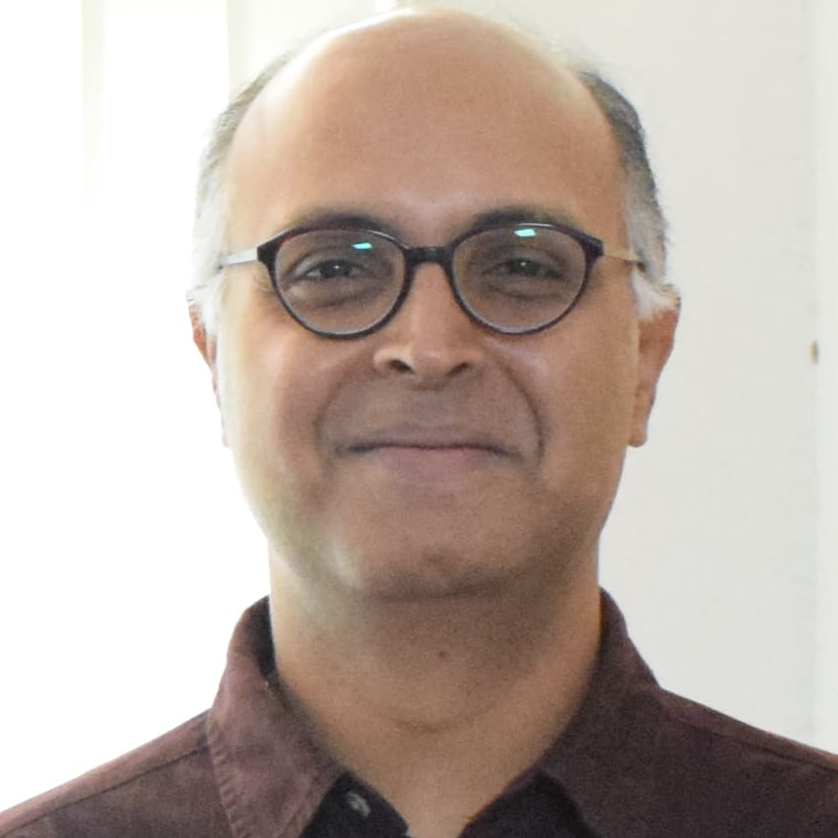
\includegraphics[width=0.6\textwidth]{slal.jpg}\\
	\footnotesize{{\bf Siddhartha Lal}\\
	IISER K}
\end{minipage}
\begin{minipage}{0.25\textwidth}
	\centering
	
\includegraphics[width=0.6\textwidth]{amukherjee.jpg}\\
	\footnotesize{{\bf Anirban Mukherjee}\\
	IISER K (Graduated)}
\end{minipage}
\begin{minipage}{0.25\textwidth}
	\centering
	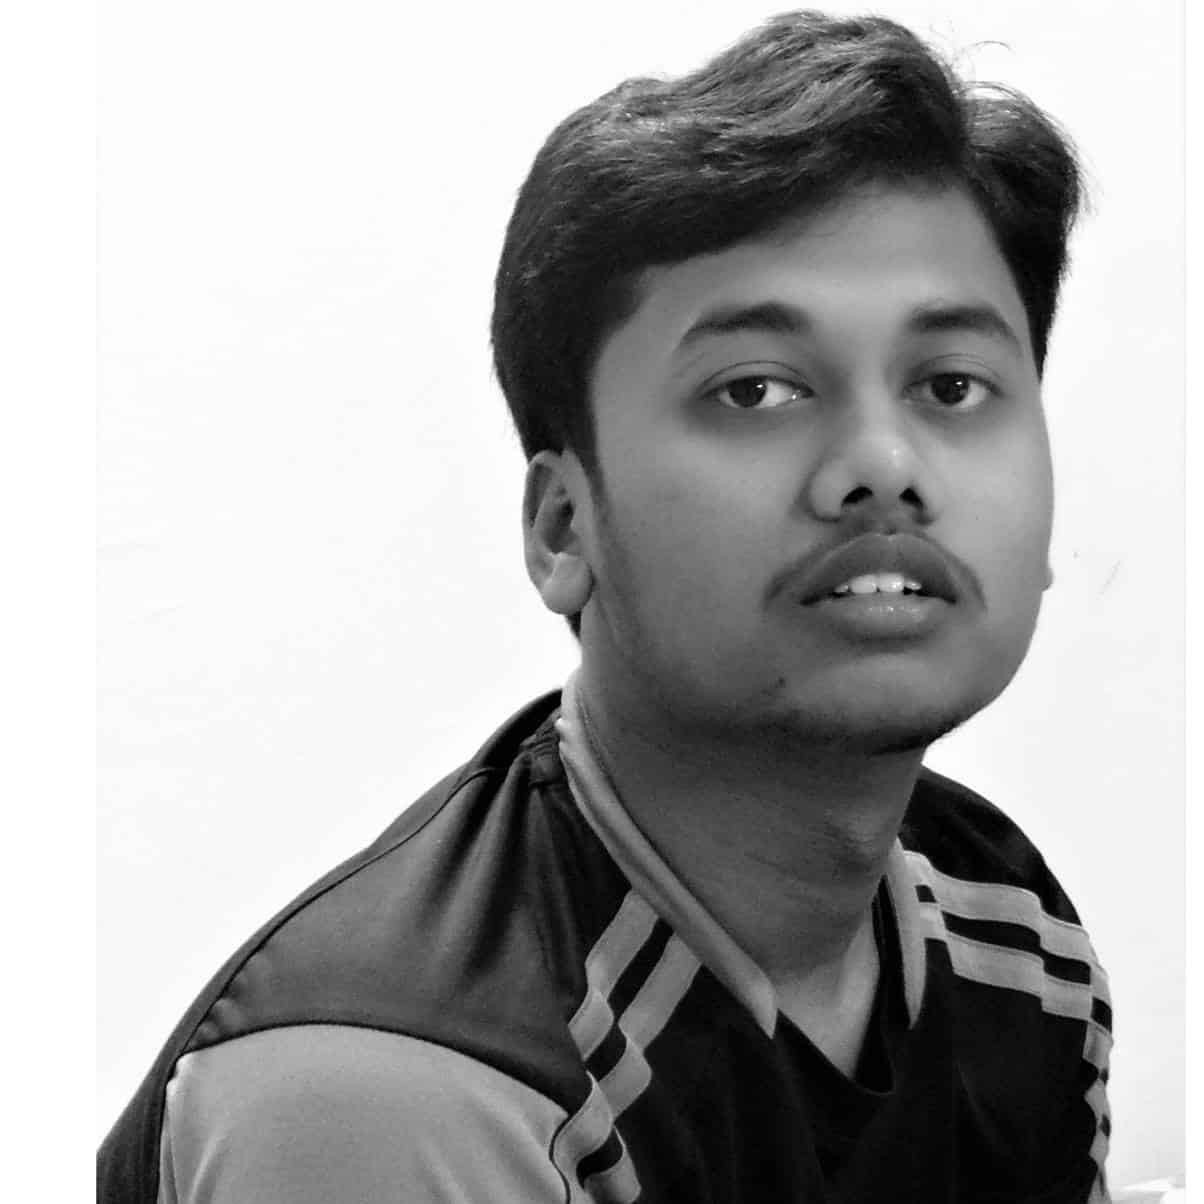
\includegraphics[width=0.6\textwidth]{spatra.jpg}\\
	\footnotesize{{\bf Siddhartha Patra}\\
	IISER K (Graduated)}
\end{minipage}
\begin{minipage}{0.1\textwidth}
	
\includegraphics[width=\textwidth]{dps_logo.jpeg}
\end{minipage}
\hspace*{\fill}
\\
\vspace*{\fill}
\alert{$\sim\sim\sim\sim\sim\sim\sim\sim\sim\sim\sim\sim\sim\sim\sim$ }\\
\alert{A huge thanks to all my collaborators! }\\
\alert{$\sim\sim\sim\sim\sim\sim\sim\sim\sim\sim\sim\sim\sim\sim\sim$ }\\
\vspace*{\fill}

\hspace*{\fill}
\begin{minipage}{0.1\textwidth}
	
\includegraphics[width=\textwidth]{IITKGP.png}\\
\end{minipage}
\hspace*{\fill}
\begin{minipage}{0.3\textwidth}
	\centering
	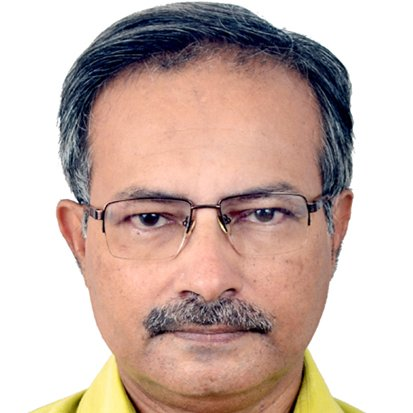
\includegraphics[width=0.45\textwidth]{arghya.jpg}\\
	\footnotesize{{\bf Arghya Taraphder}\\
	IIT Kharagpur}
\end{minipage}
\hspace*{\fill}
\begin{minipage}{0.3\textwidth}
	\centering
	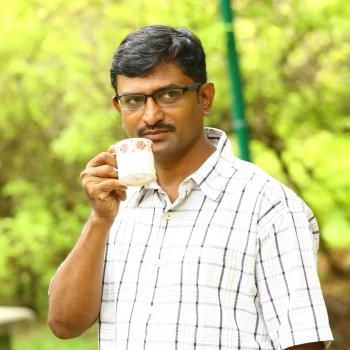
\includegraphics[width=0.45\textwidth]{nsv.jpeg}\\
	\footnotesize{{\bf N. S. Vidhyadhiraja}\\
	JNCASR Bangalore}
\end{minipage}
\hspace*{\fill}
\begin{minipage}{0.1\textwidth}
	
\includegraphics[width=\textwidth]{JNCASR.png}\\
\end{minipage}
\hspace*{\fill}

\end{frame}

\section{Introducing the Kondo effect}
\subsection{Where it all began}

\begin{frame}{What is the Kondo effect?}
\begin{minipage}{0.5\textwidth}
\begin{itemize}
	\item metal resistivity is \alert{monotonic}: \(\rho \sim T^n\)\\[10pt]
	\item dilute alloys show anomalous \alert{minimum}\\[10pt]
	\item resistivity eventually becomes \alert{constant}
\end{itemize}
\end{minipage}
\hspace*{\fill}
\begin{minipage}{0.45\textwidth}
\centering
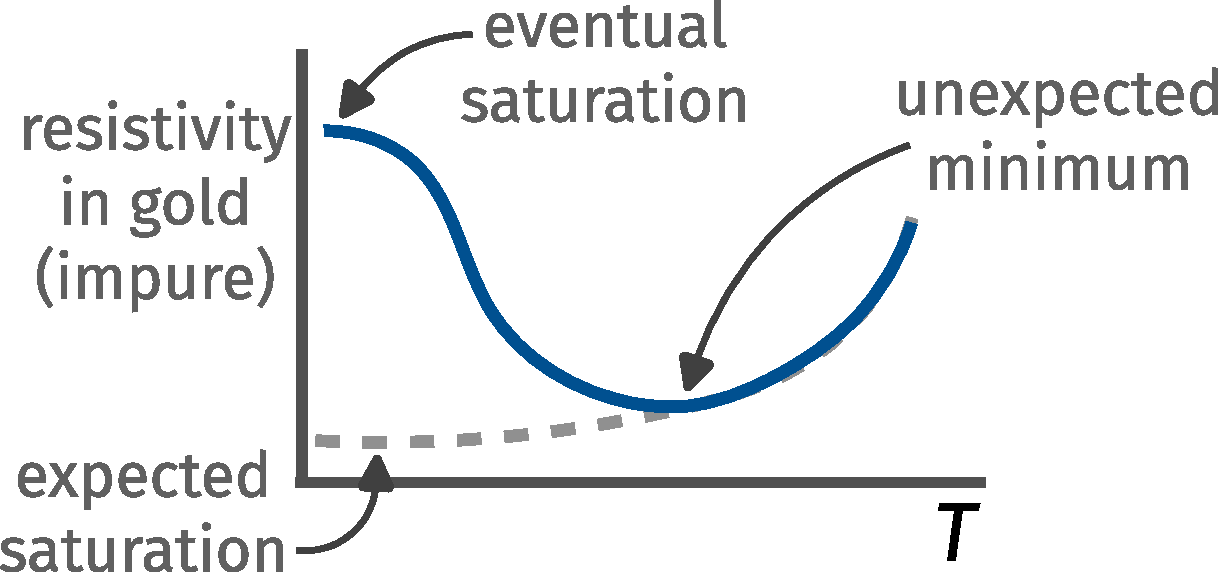
\includegraphics[width=\textwidth]{resistance_minimum.pdf}
\end{minipage}

\[\text{Can be explained using the \alert{Kondo model}:}\quad H_\text{Kondo} = KE_\text{bath} + J \vec{S}_\text{imp}\cdot\vec{S}_\text{bath}\]

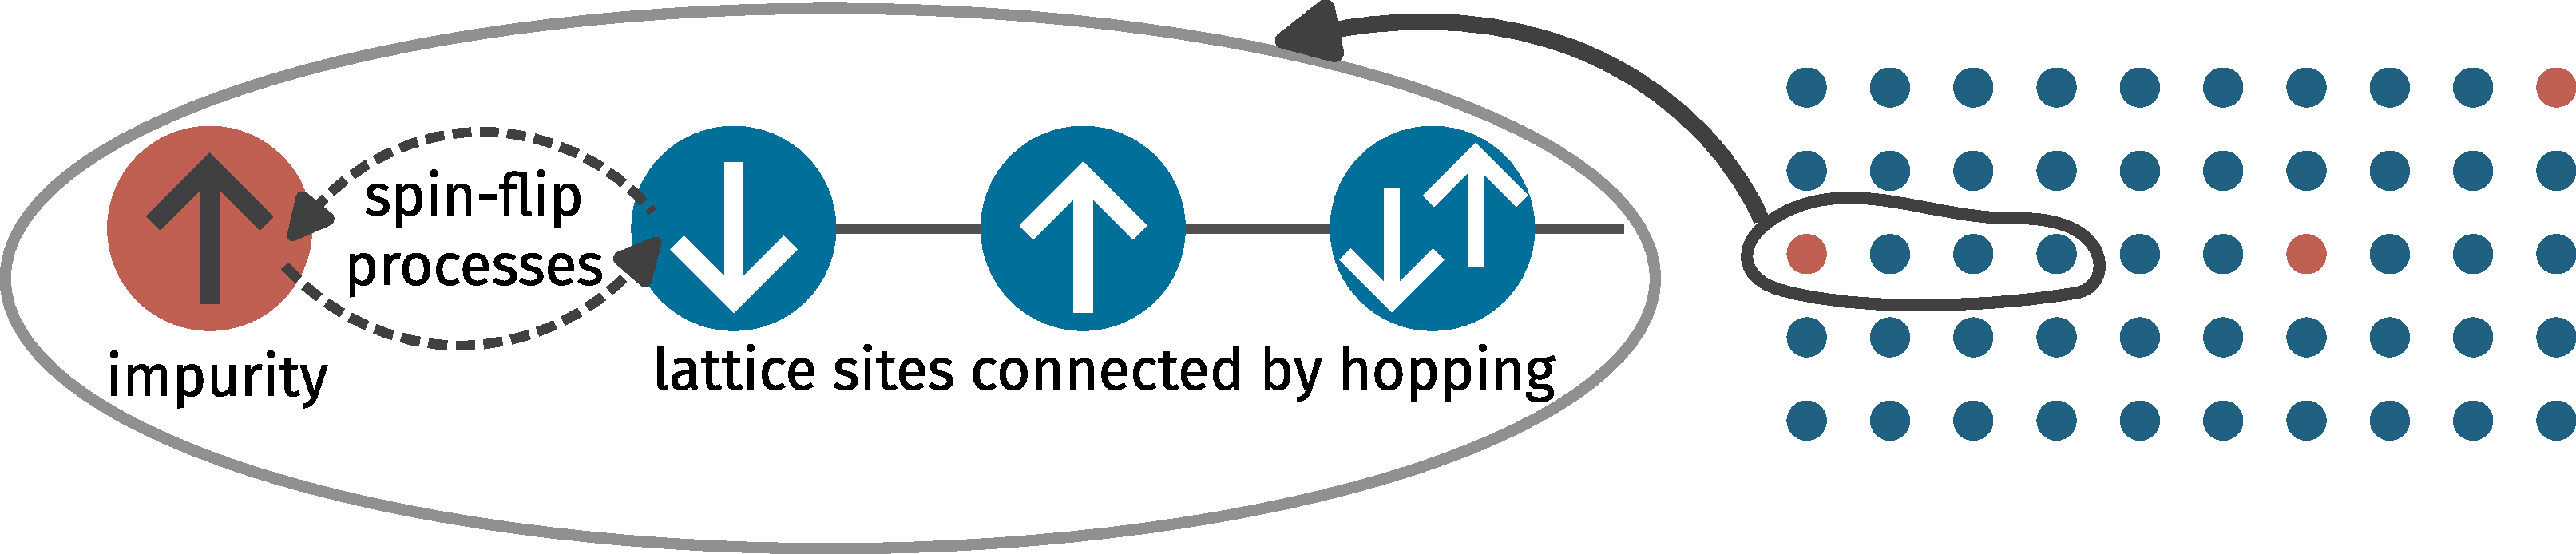
\includegraphics[width=0.9\textwidth]{KondoModel.pdf}

\footcite{deHaas1939,Sarachik1964,Heeger1969}
\end{frame}

\begin{frame}{How to explain the resistance minimum \& eventual saturation?}
\footcite{kondo1964resistance}
\begin{minipage}{0.5\textwidth}
Second order perturbation theory in \(J\) gives:
\[\hspace*{-80pt}\rho \sim T^n - \ln T\]
Explains the \alert{non-monotonic}\\
behaviour!\\[20pt]
However, solution \alert{diverges} at \(T \to 0\)!
\end{minipage}
\begin{minipage}{0.4\textwidth}
	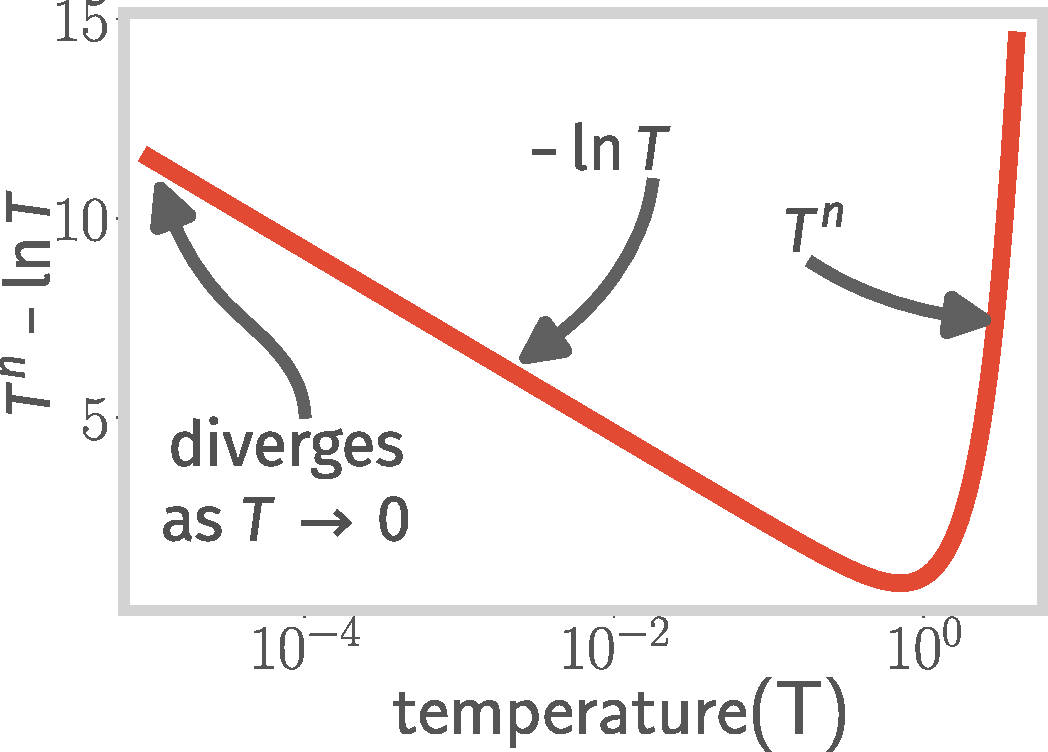
\includegraphics[width=\textwidth]{secondorder.pdf}
\end{minipage}
\begin{textblock*}{0.13\textwidth}(6.5cm, 3.8cm)
	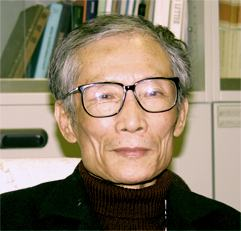
\includegraphics[width=\textwidth]{kondo.jpg}\\
	\footnotesize{(Jun Kondo)}
\end{textblock*}
\end{frame}

\begin{frame}{How to explain the resistance minimum \& eventual saturation?}
\footcite{wilson1975,andrei_1980,Wiegmann_1981,affleck1995conformal}
Breakdown of perturbation theory indicates a \alert{change in ground state}!\\[10pt]
Obtaining \(T=0\) ground state requires more \alert{powerful  methods}\\[10pt]

\begin{minipage}{0.2\textwidth}
\centering
Numerical RG\\[10pt]
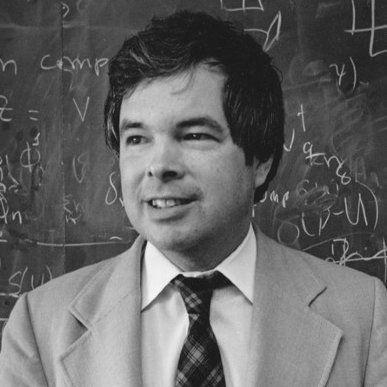
\includegraphics[width=0.5\textwidth]{wilson.jpg}\\
\footnotesize{(K. G. Wilson)}
\end{minipage}
\begin{minipage}{0.2\textwidth}
\centering
Bethe ansatz\\[10pt]
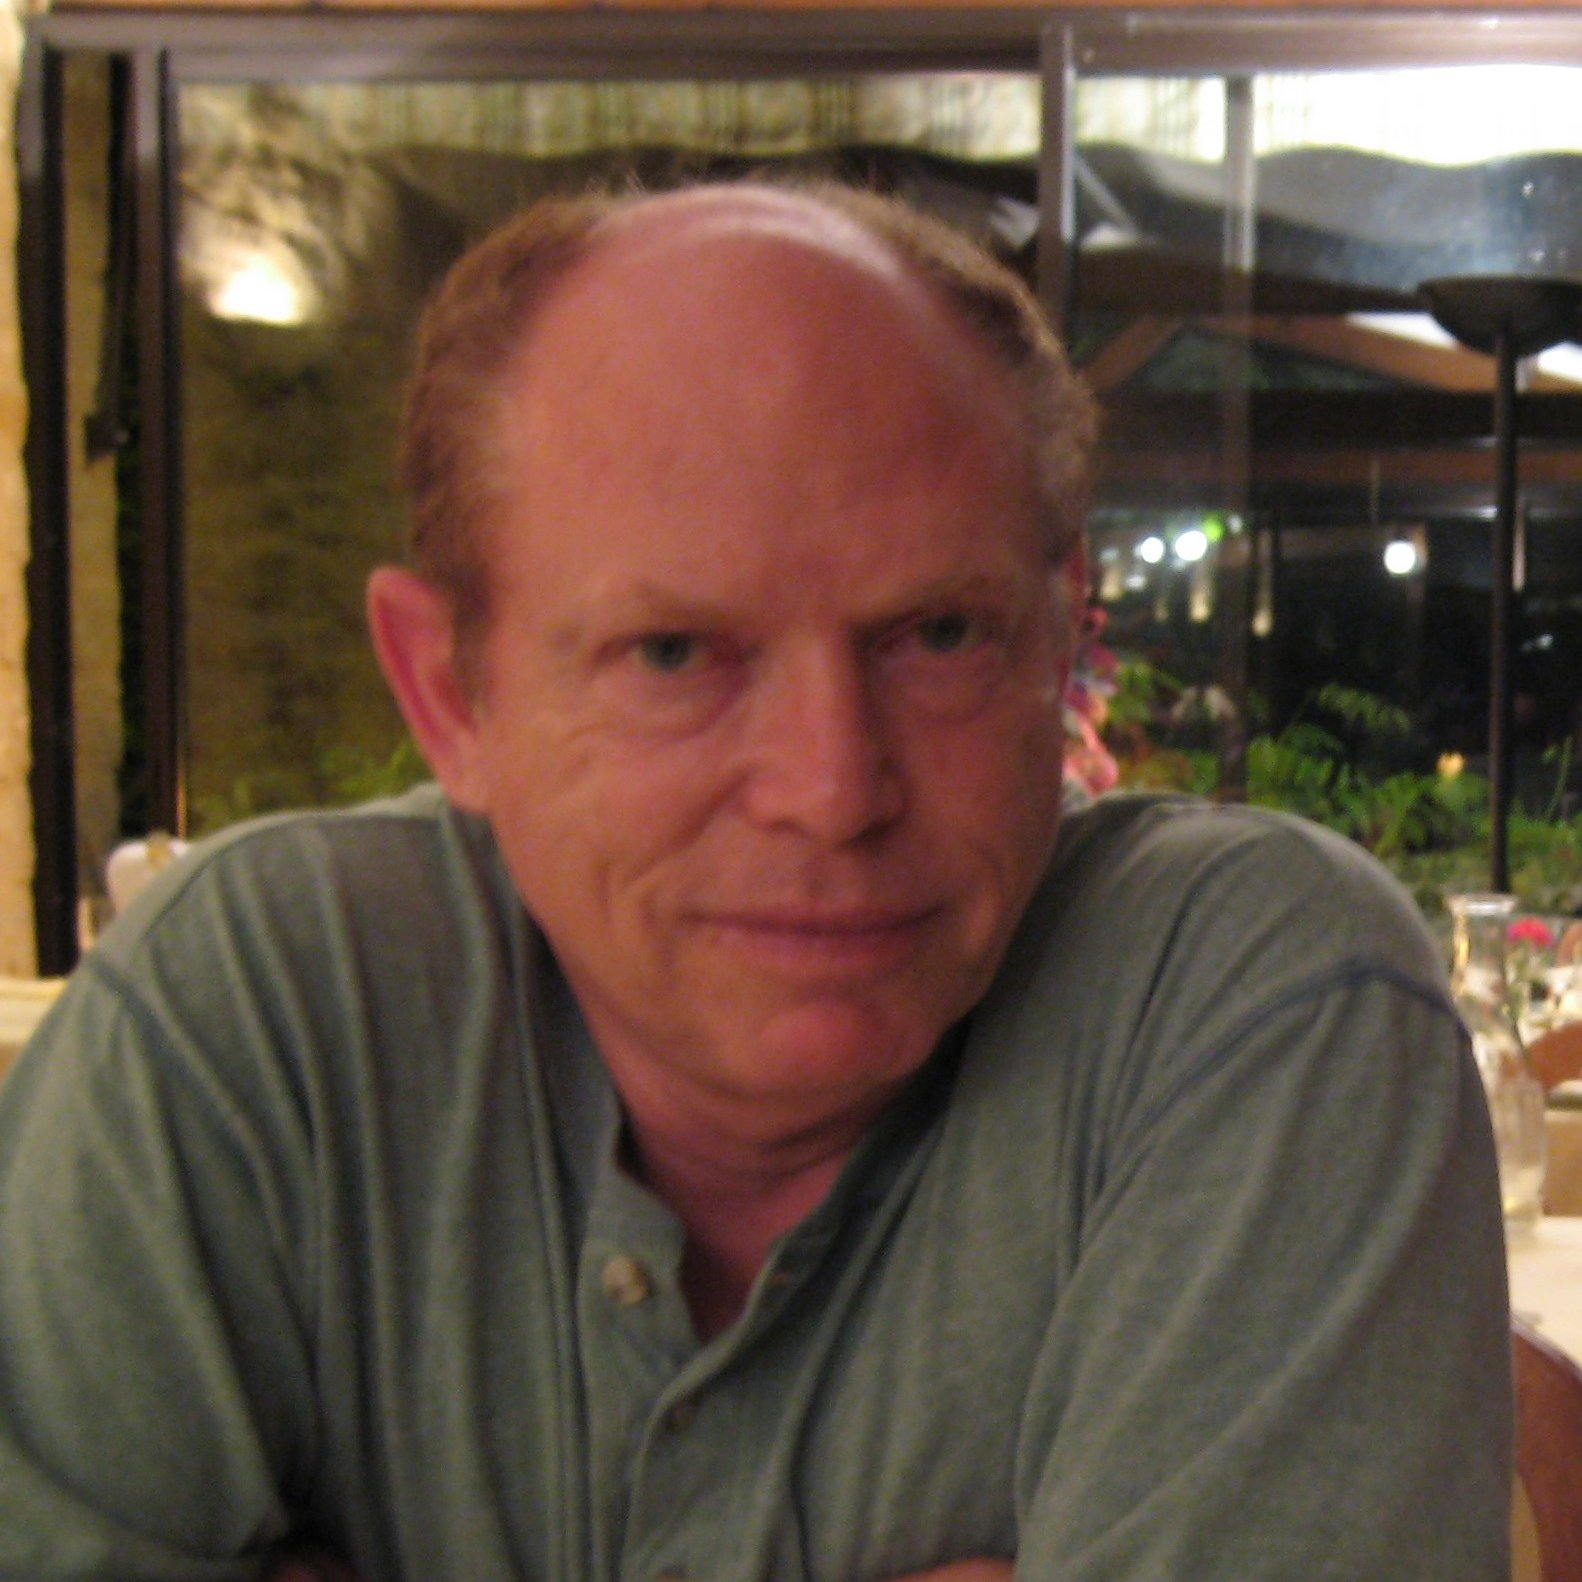
\includegraphics[width=0.5\textwidth]{AndreiN.jpg}\\
\footnotesize{(Natan Andrei)}
\end{minipage}
\begin{minipage}{0.2\textwidth}
\centering
Conf. field theory\\[10pt]
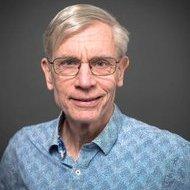
\includegraphics[width=0.5\textwidth]{affleck.jpg}\\
\footnotesize{(Ian Affleck)}
\end{minipage}
\begin{minipage}{0.38\textwidth}
\begin{itemize}
	\item impurity becomes \alert{strongly coupled} at low temperatures
	\item local moment crosses over into \alert{nonmagnetic} singlet
\end{itemize}
\end{minipage}

\vspace*{\fill}
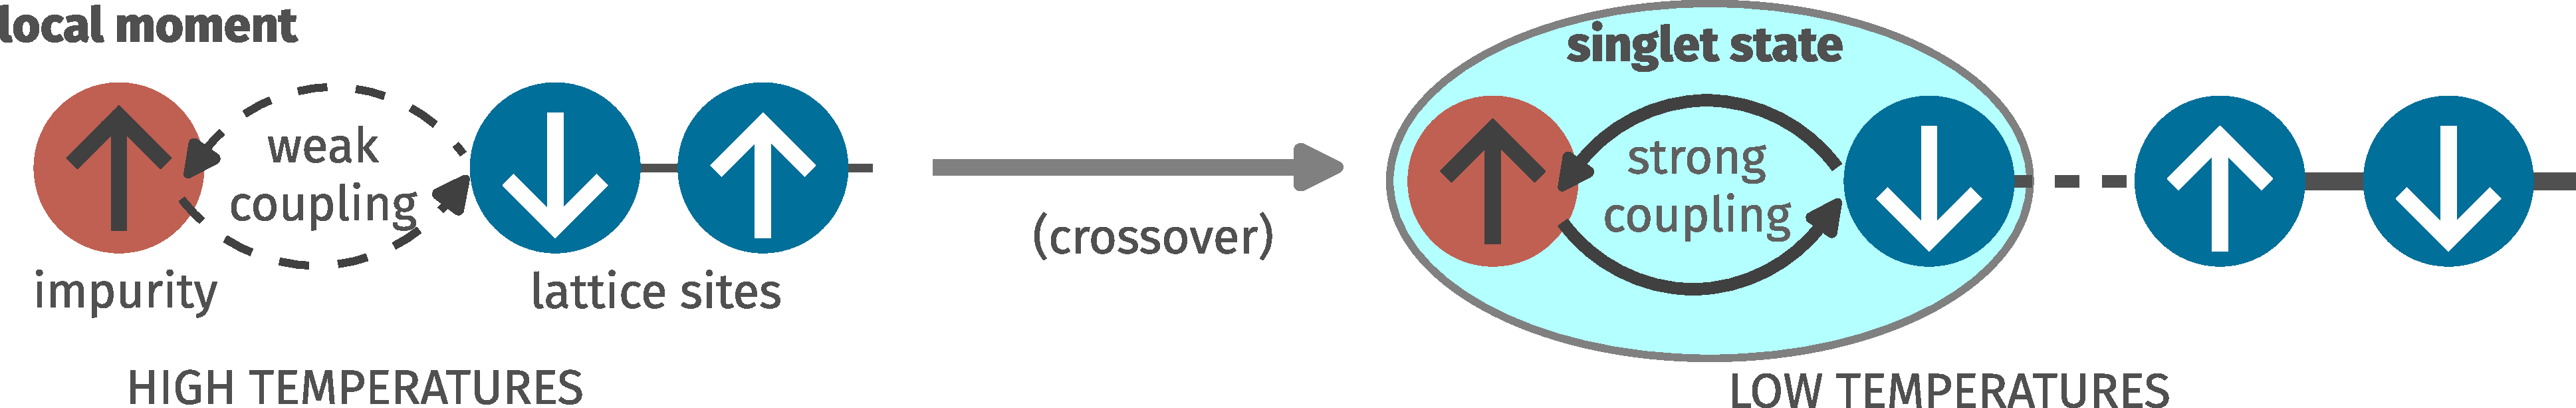
\includegraphics[width=0.9\textwidth]{crossover.pdf}\\

\end{frame}

\section{Some important questions}
\begin{frame}{Some important questions}
\begin{minipage}{0.45\textwidth}
	1. How do we describe the dynamics of the electrons that screen the impurity (the so-called \alert{Kondo cloud})?
\end{minipage}
\hspace*{\fill}
\begin{minipage}{0.45\textwidth}
	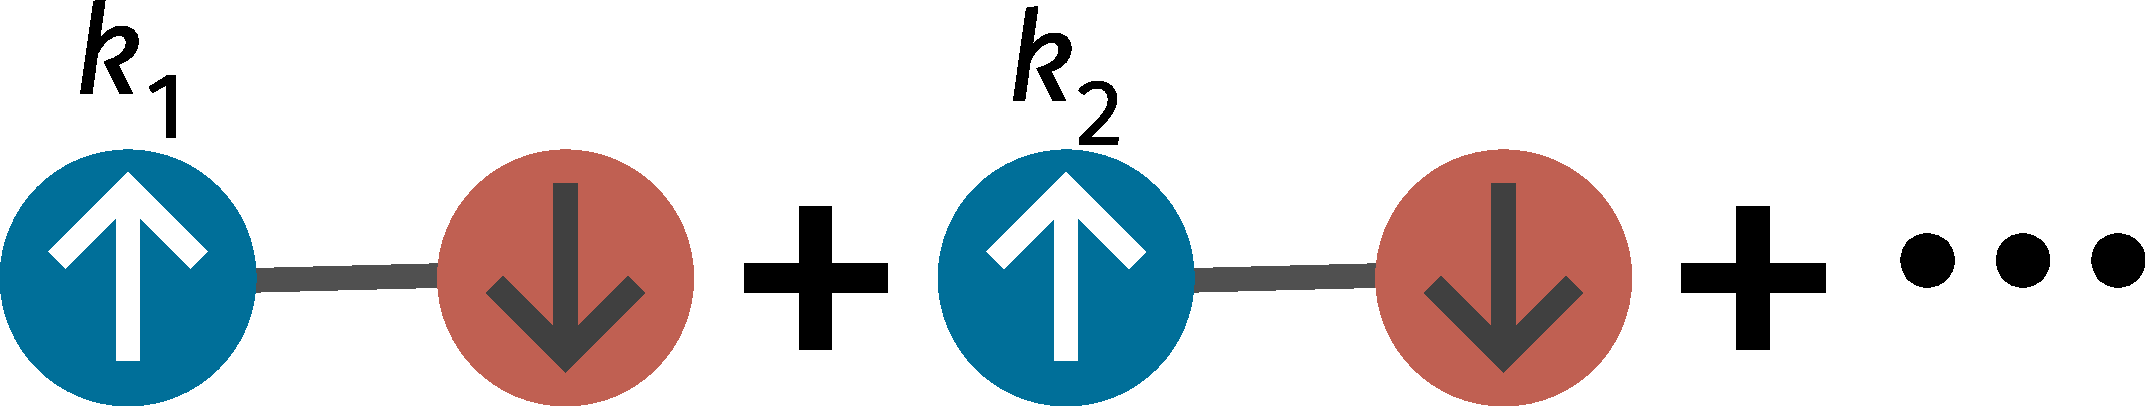
\includegraphics[width=0.9\textwidth]{kondocloud.pdf}
\end{minipage}
\vspace*{\fill}

\begin{minipage}{0.45\textwidth}
	
\includegraphics[width=0.9\textwidth]{distortsinglet.pdf}
\end{minipage}
\hspace*{\fill}
\begin{minipage}{0.45\textwidth}
	2. What kind of physics can \alert{disturb the Kondo screening} effect and distort the singlet state?
\end{minipage}
\vspace*{\fill}

\begin{minipage}{0.45\textwidth}
	3. What is the simplest impurity model that completely destroys the Kondo effect and leads to a \alert{phase transition}?
\end{minipage}
\hspace*{\fill}
\begin{minipage}{0.45\textwidth}
	
\includegraphics[width=0.9\textwidth]{kondobreakdown.pdf}
\end{minipage}
\end{frame}

\section{The single-channel Kondo problem:\\ Anatomy of the Kondo cloud}
\begin{textblock*}{\textwidth}(1cm, 4.5cm)

\includegraphics[width=\textwidth]{kondocloud_prb.pdf}\\
\end{textblock*}
\subsection{~}

\begin{frame}{Unitary RG approach to impurity models}
\footcite{anirbanurg1,anirbanurg2}
\begin{minipage}{0.5\textwidth}
\begin{itemize}
	\item Integrate out \alert{high energy fluctuations} to reach strong-coupling low-energy theory\\[10pt]
	\item Leads to \alert{singlet ground state} and decoupled high-energy \(k-\)states\\[10pt]
	\item Decoupling is carried out through \alert{unitary transformations}
\end{itemize}

\end{minipage}
\hspace*{\fill}
\begin{minipage}{0.4\textwidth}
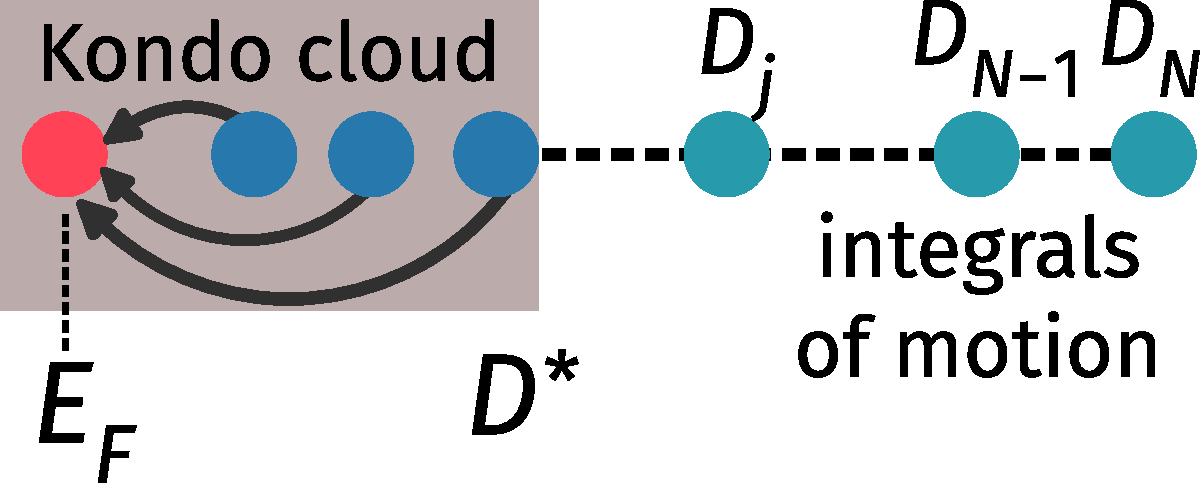
\includegraphics[width=\textwidth]{kondo_fp_1D.pdf}
\end{minipage}
	
\end{frame}

\begin{frame}{Effective Hamiltonian for the Kondo cloud}
\footcite{anirban_kondo}
In order to obtain a theory for the Kondo cloud,\\ we \alert{trace out impurity} from fixed point Hamiltonian.
\vspace*{\fill}

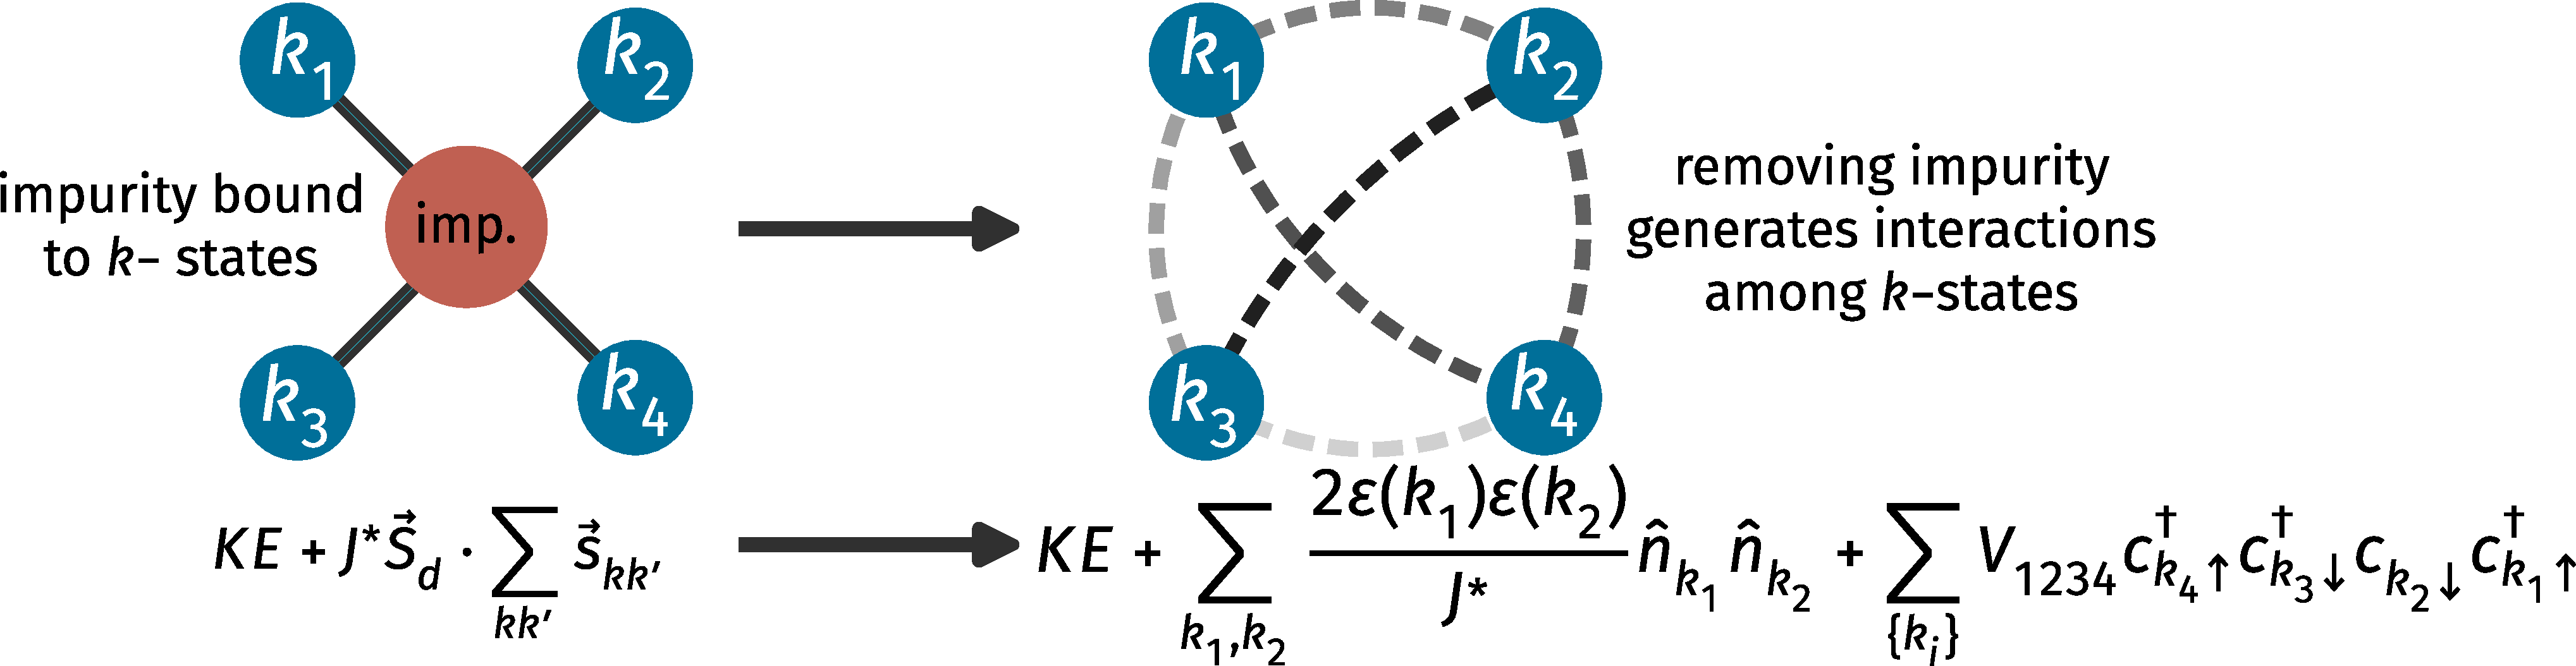
\includegraphics[width=\textwidth]{KondoCloud.pdf}

\vspace*{\fill}
\begin{itemize}
	\item all-to-all interactions between momentum states, \alert{large entanglement}
	\item 2-particle interaction terms \alert{not} present in Fermi liquid, are \alert{responsible for screening}
\end{itemize}

\end{frame}

\begin{frame}{Quantifying entanglement within the Kondo cloud}
\only<1-2>{
\begin{minipage}{0.8\textwidth}
In order to demonstrate formation of Kondo cloud, we study the \alert{variation of entanglement} and correlations under RG transformations.
\end{minipage}

\vspace*{\fill}
\begin{itemize}[<+->]
	\item Entanglement entropy \(S(A)\) \(\Longrightarrow\) quantifies how much \alert{information is gained} about the rest of the system by measuring \(A\)\\
	\vspace*{\fill}
	{\centering
	\only<1>{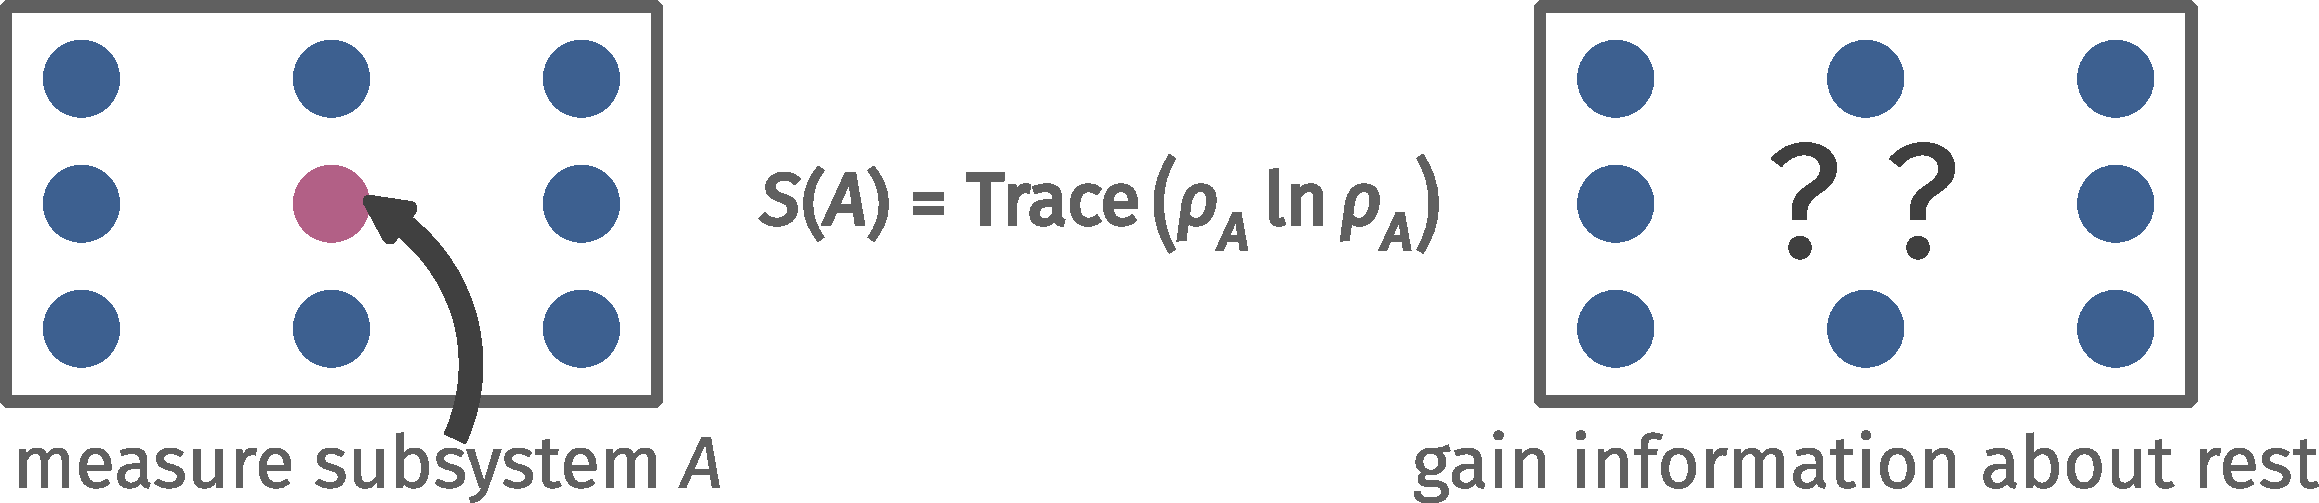
\includegraphics[width=0.85\textwidth]{entanglement.pdf}}}
\item Mutual information \(I_2(A:B)\)\(\Longrightarrow\) quantifies how much \alert{information about subsystem A} is gained by measuring \(B\)\\
	\vspace*{\fill}
	{\centering
	\only<2>{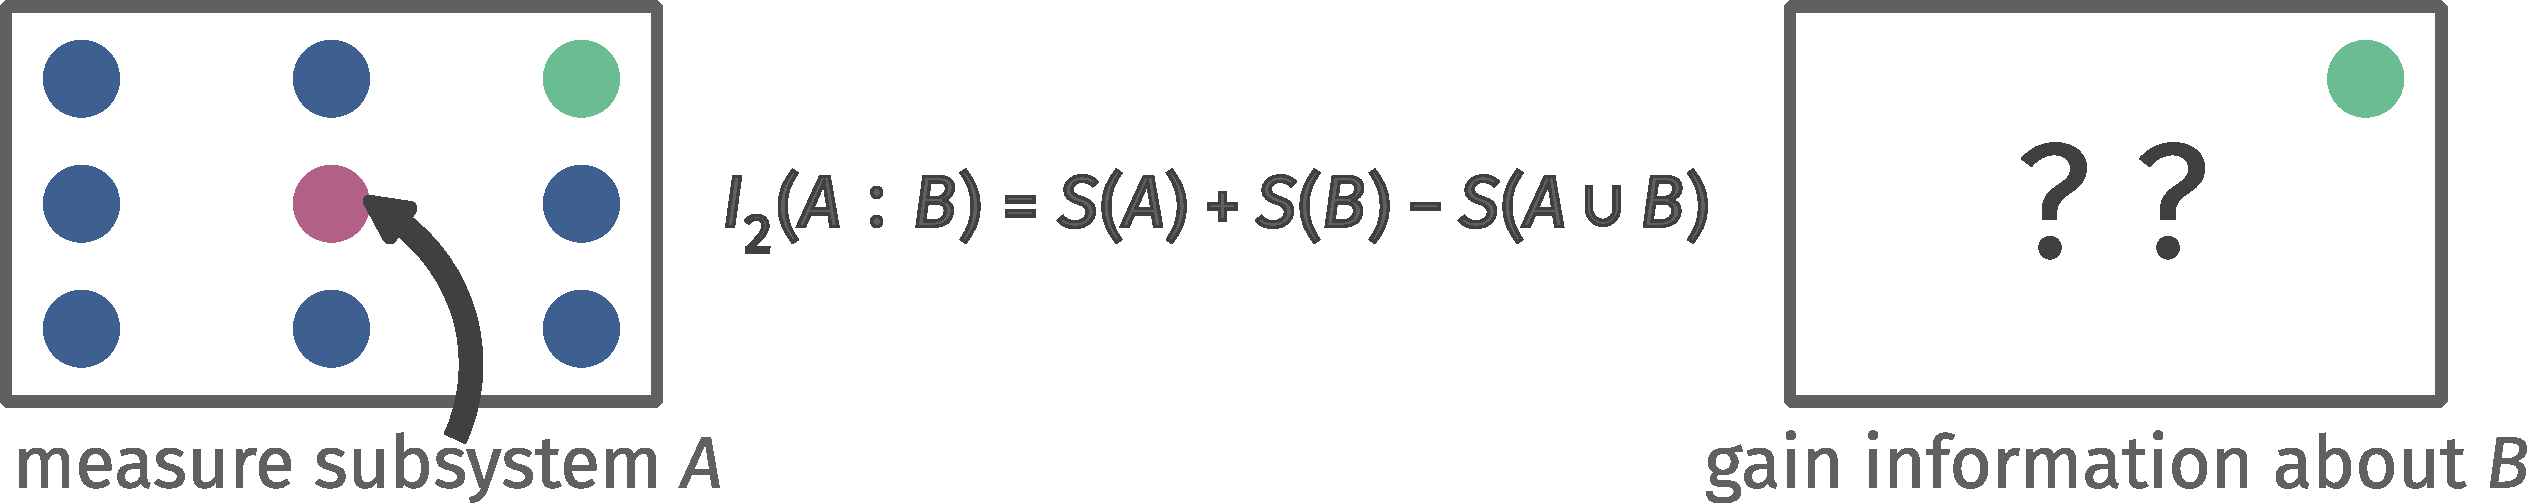
\includegraphics[width=0.85\textwidth]{mutinfo.pdf}}}
\end{itemize}
}
\only<3>{
\footcite{anirban_kondo}
Both entanglement and \(k-\)space correlations \alert{increase} as RG proceeds from UV to IR.

\vspace*{\fill}
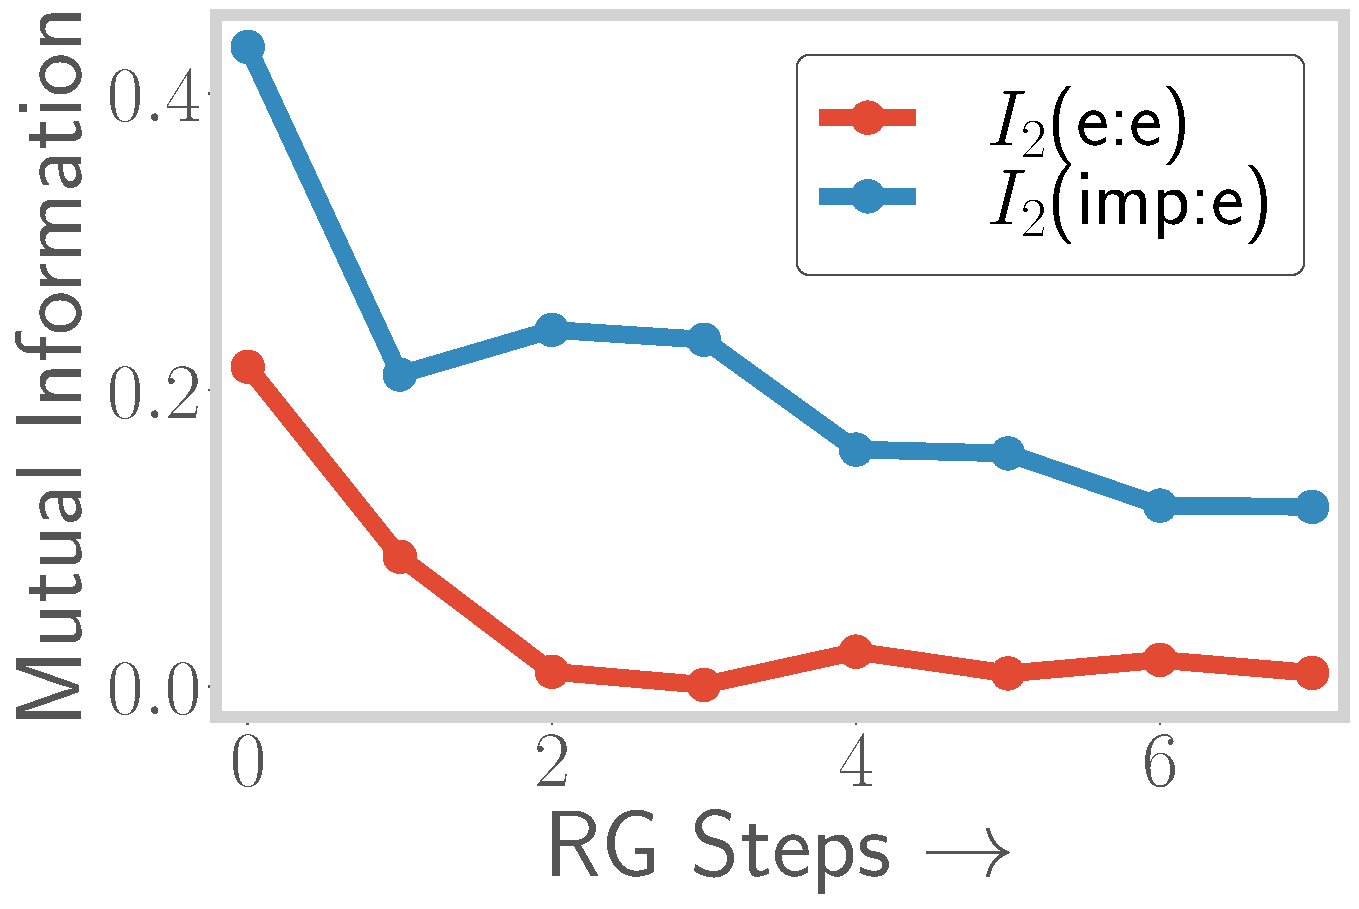
\includegraphics[width=0.4\textwidth]{MIkondo.pdf}
\hspace*{\fill}
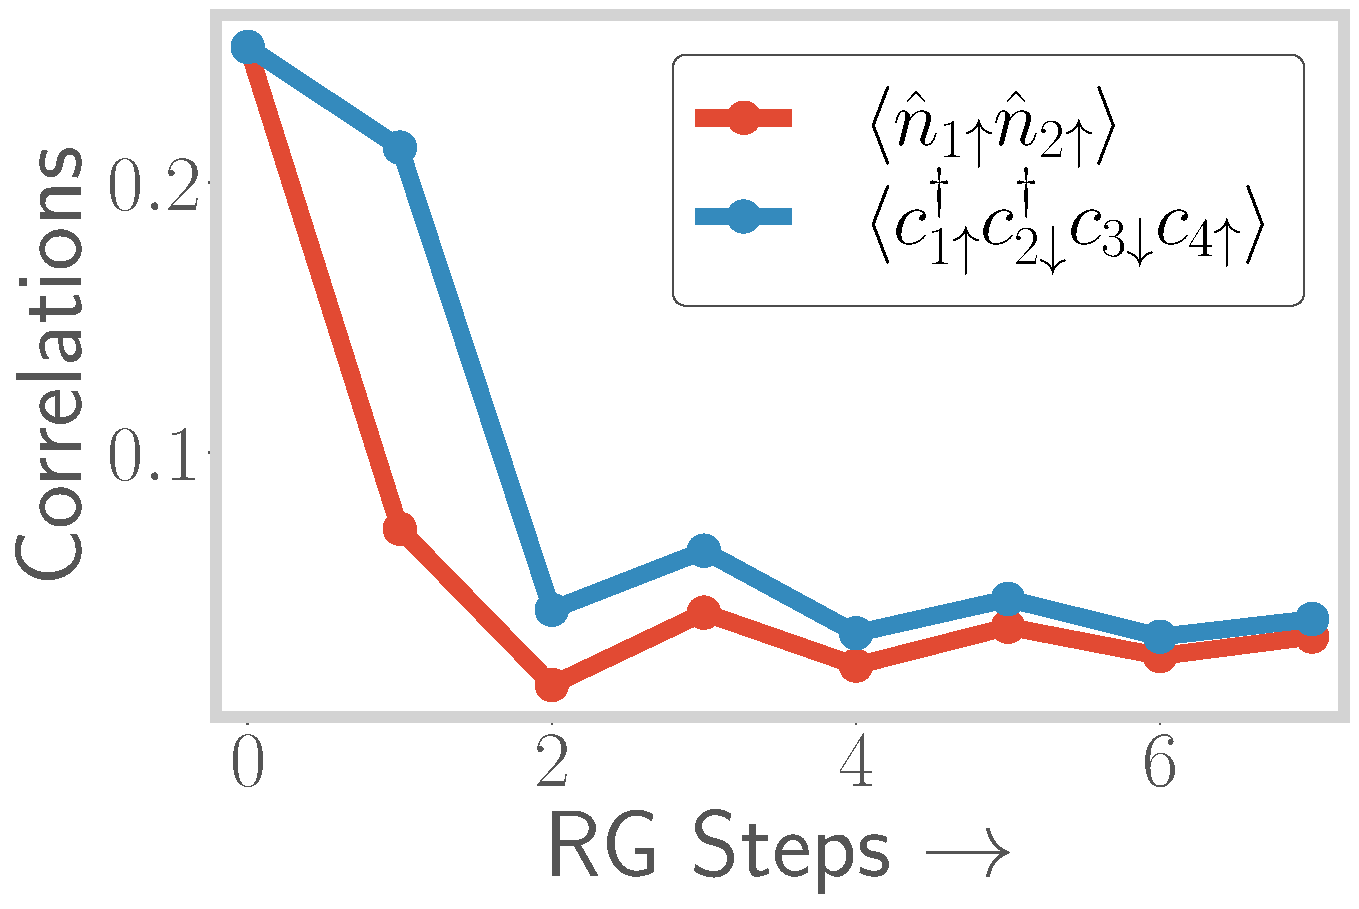
\includegraphics[width=0.4\textwidth]{corrKondo.pdf}

\vspace*{\fill}
\begin{itemize}
	\item The former shows the formation of the \alert{Kondo singlet}\\[10pt]
	\item The latter shows the growth of two-particle correlations in the \alert{Kondo cloud}
\end{itemize}
}
\end{frame}

\section{Distorting the Kondo singlet:\\ The multi-channel Kondo Problem}
\begin{textblock*}{\textwidth}(1cm, 4.1cm)

\includegraphics[width=0.9\textwidth]{MCKJPCM.pdf}
\end{textblock*}
\subsection{~}

\begin{frame}{What is the multichannel Kondo problem?}
\footcite{Noz_blandin_1980,affleck1993exact,emery_kivelson,andrei_destri_1984}
\begin{minipage}{0.39\textwidth}
Single impurity interacting with \alert{multiple channels} in the bath
\[H_\text{Kondo} = KE_\text{bath} + \sum_{l}J_l \vec{S}_\text{imp}\cdot\vec{s}^{(l)}\]
Known to display divergent impurity susceptibility as \(T \to 0\), indicating \alert{incomplete screening}
\end{minipage}
\hspace*{\fill}
\begin{minipage}{0.45\textwidth}
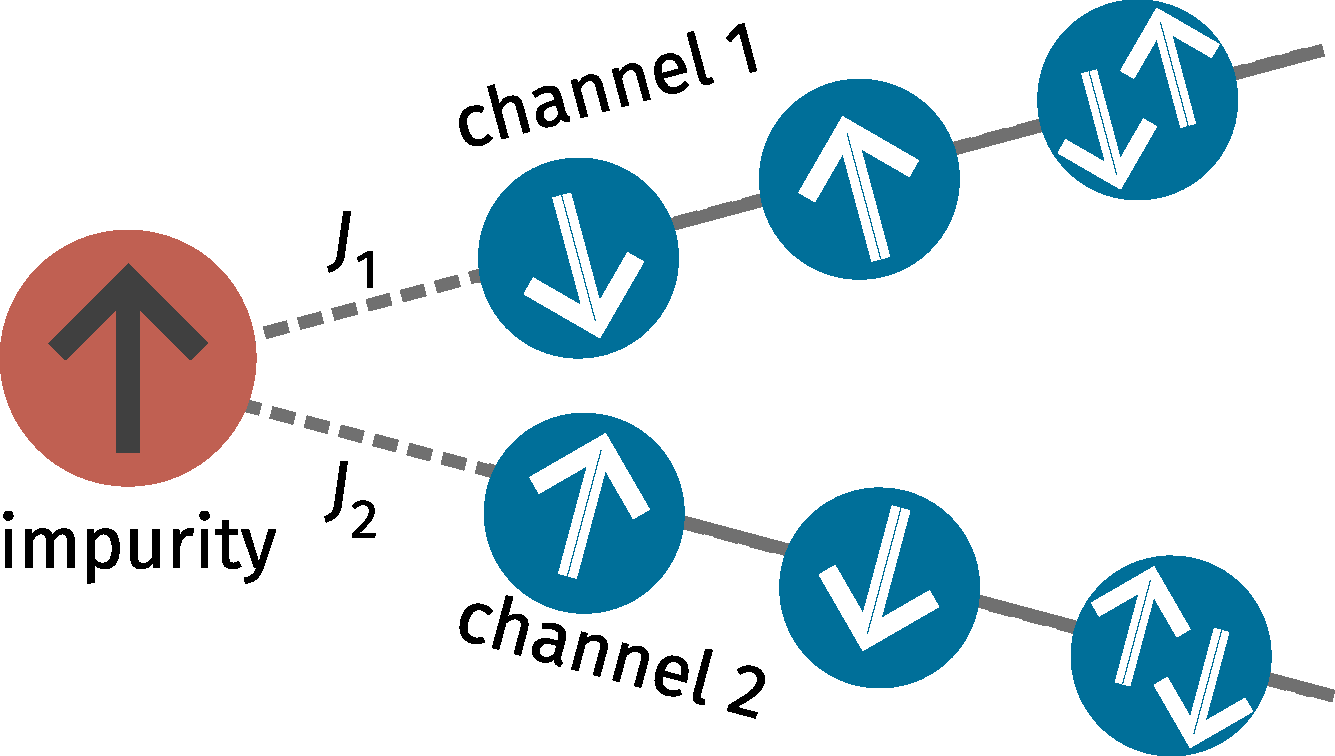
\includegraphics[width=\textwidth]{MCKM.pdf}
\end{minipage}
\vspace*{\fill}

Other anomalous features: orthogonality catastrophe, \alert{non-Fermi liquid} excitations, diverging specific heat
\end{frame}

\begin{frame}{Can a simpler model make this more intuitive?}
\footcite{Patra_2023}
\only<1>{
\begin{minipage}{0.45\textwidth}
At \(T=0\) and in the ground state, consider \alert{only} lowest energy state in bath.
\end{minipage}
\hspace*{\fill}
\begin{minipage}{0.45\textwidth}
	\[KE_\text{bath} + \sum_{l=1}^K J_l \vec{S}_\text{imp}\cdot\vec{s}^{(l)} \Longrightarrow \sum_{l=1}^K J_l \vec{S}_\text{imp}\cdot\vec{s_0}^{(l)} \]
\end{minipage}

\vspace*{\fill}
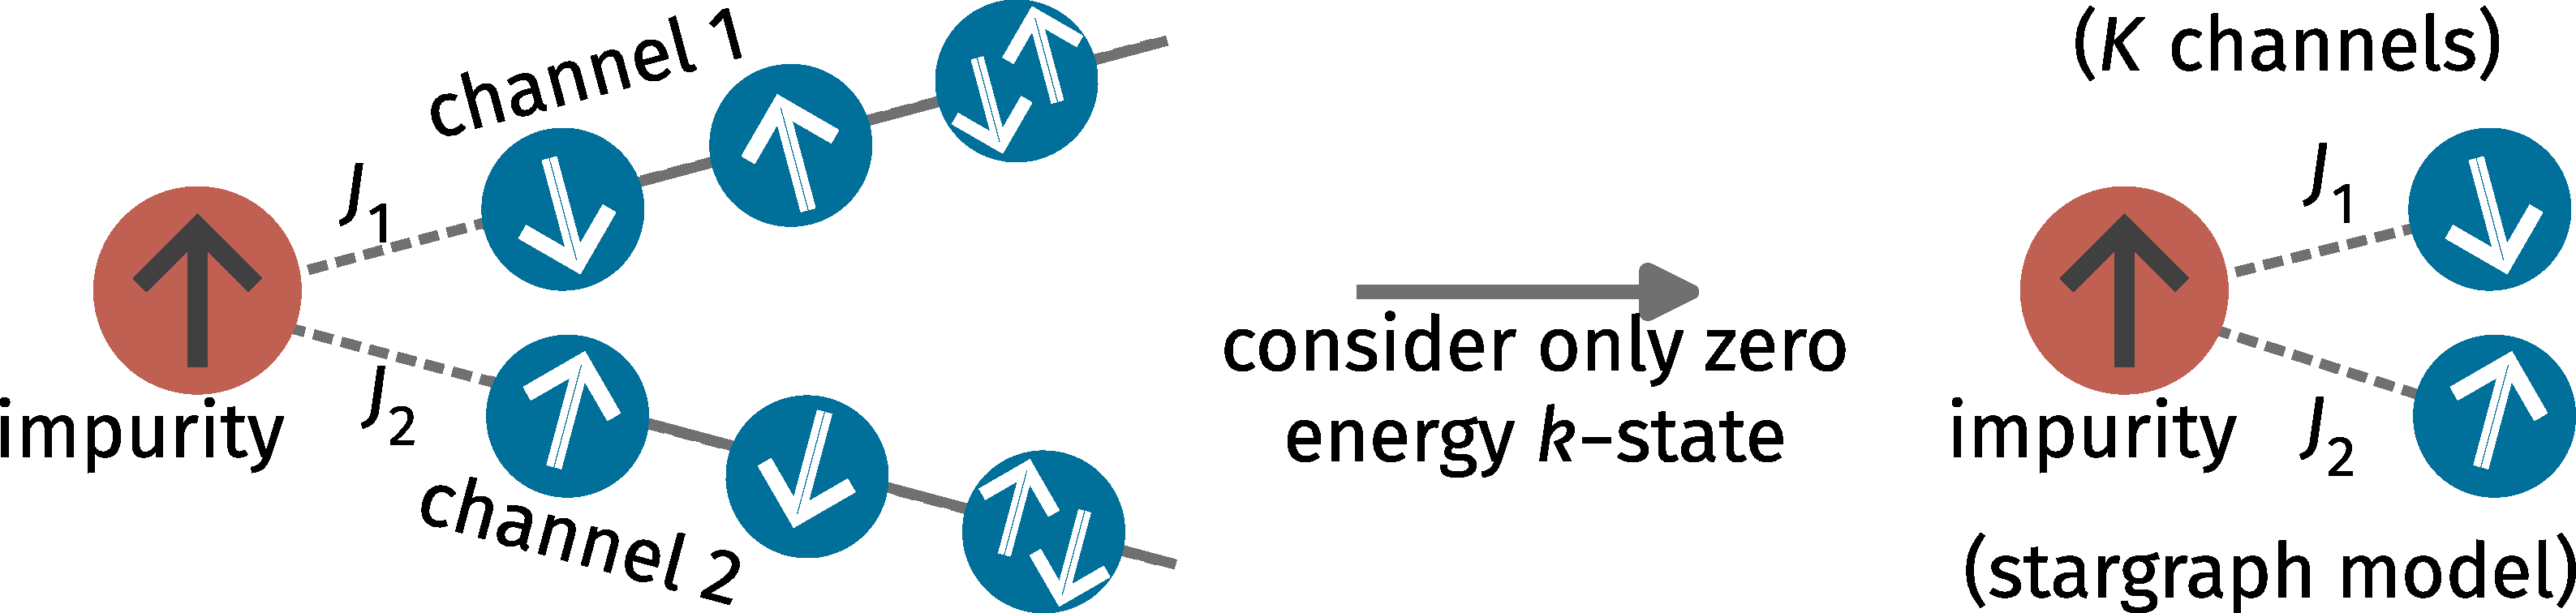
\includegraphics[width=0.7\textwidth]{MCKM_zeroB.pdf}
}
\only<2>{
\begin{minipage}{0.7\textwidth}
\[\text{Model is (analytically) solvable}: \left\{\ket{S_\text{tot}^z}\right\}\]
\[\text{Ground state is \alert{degenerate} for $K > 1$}\]
\begin{itemize}
	\item Degeneracy for \(K > 1\) shows orthogonality catastrophe\\[10pt]
	\item \(S_\text{tot}^z \neq 0\) in ground states shows incomplete screening
\end{itemize}
\end{minipage}
\hspace*{\fill}
\begin{minipage}{0.25\textwidth}
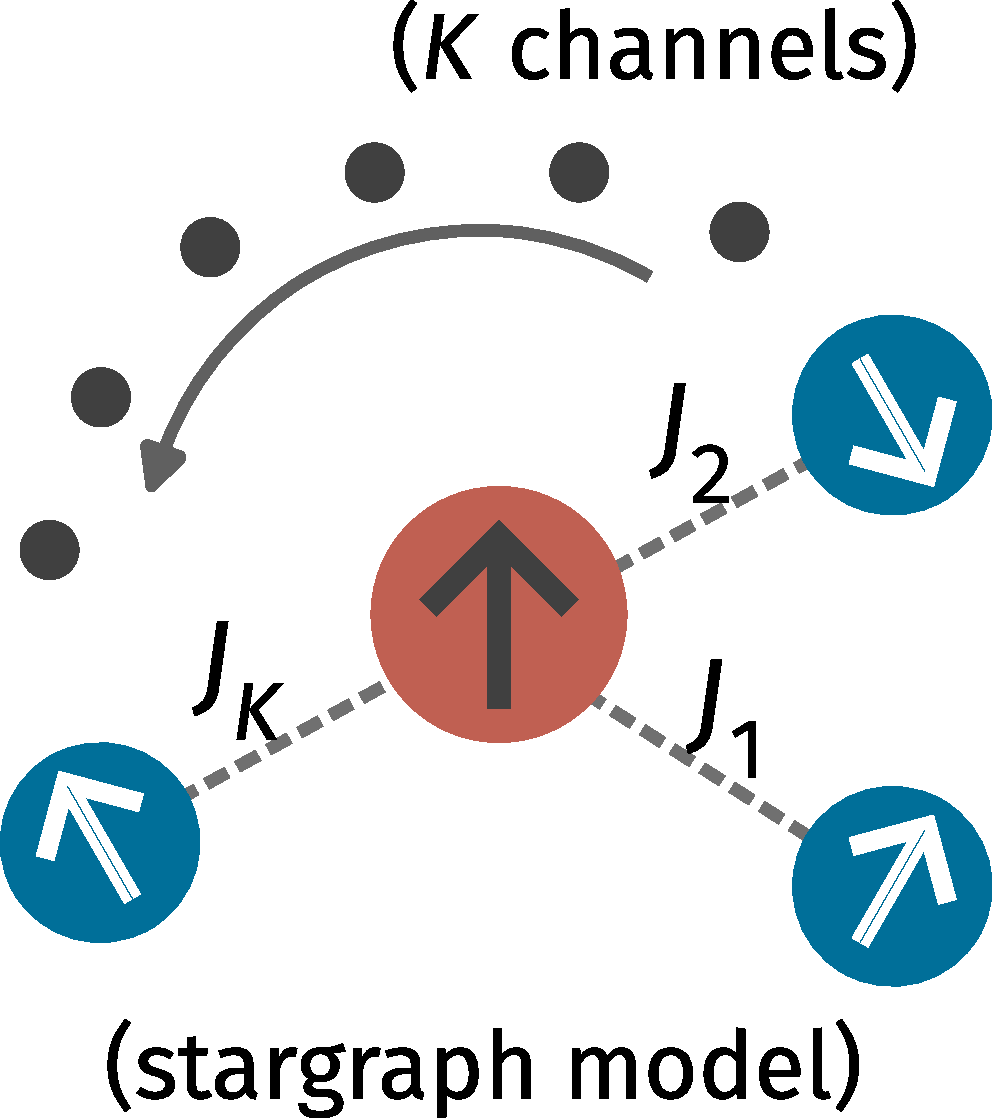
\includegraphics[width=\textwidth]{stargraph.pdf}
\end{minipage}
}
\only<3>{
\begin{minipage}{0.55\textwidth}
	Magnetisation of central node goes as 
	\[ m = \frac{1-K}{2(1 + K)}\]
\begin{itemize}
	\item Susceptibility shows \(T=0\) \alert{divergence} for \(K > 1\)\\[10pt]
	\item Magnetisation can be linked to \alert{scattering phase shifts} and hence to RG equation
\end{itemize}
\end{minipage}
\hspace*{\fill}
\begin{minipage}{0.35\textwidth}
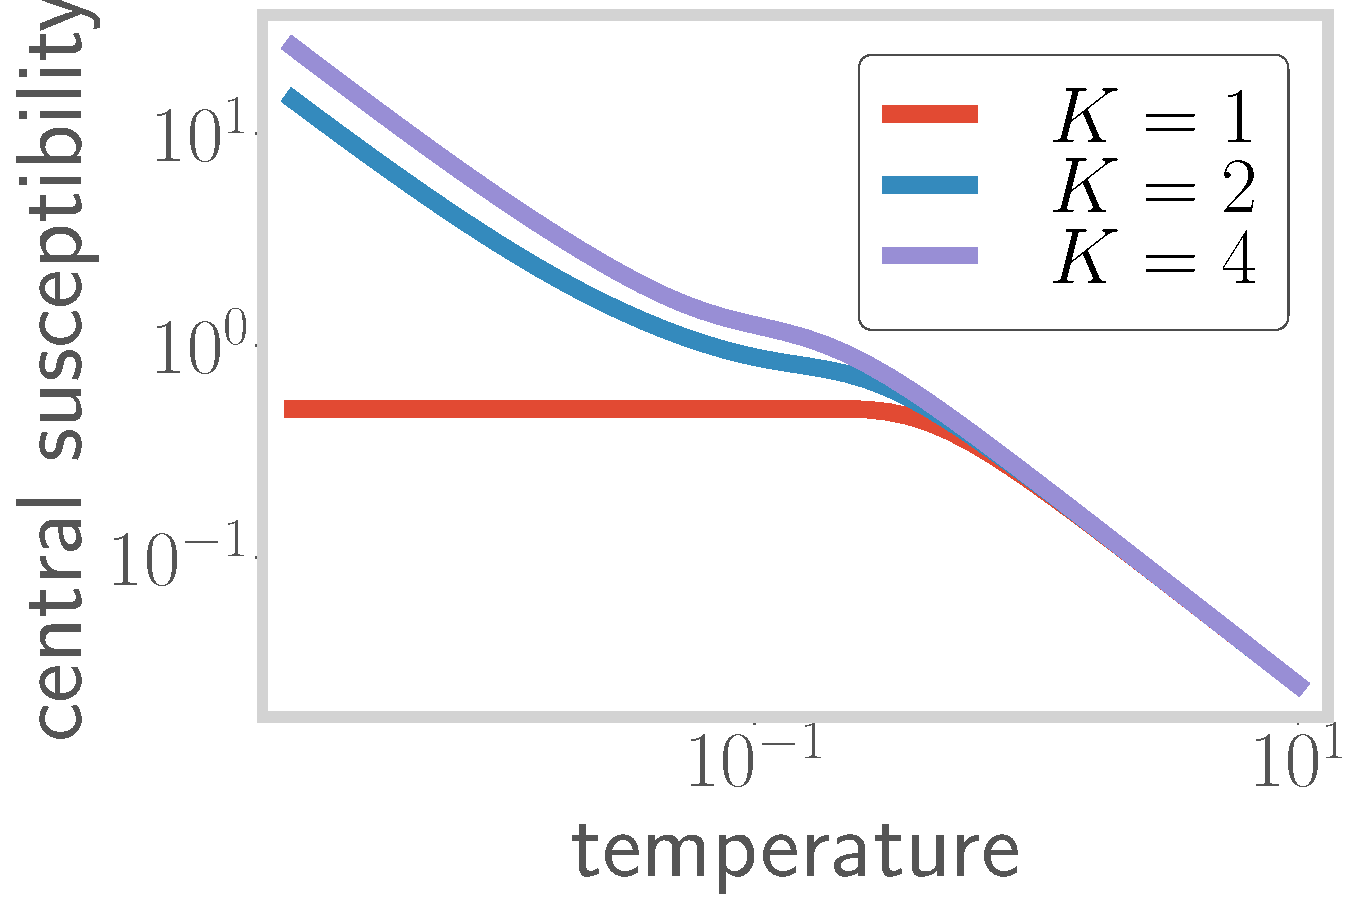
\includegraphics[width=\textwidth]{MCK_imp_chi.pdf}
\end{minipage}
}
\only<4>{
\begin{minipage}{0.4\textwidth}
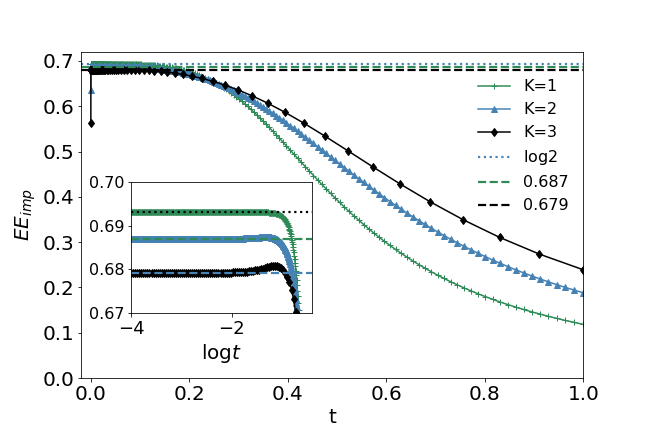
\includegraphics[width=\textwidth]{EE_excitations.png}
\end{minipage}
\hspace*{\fill}
\begin{minipage}{0.55\textwidth}
Upon including excitations above the stargraph\\
\begin{itemize}
	\item entanglement entropy of central node shows \alert{discontinuity} \(\Longrightarrow\) orthogonality catastrophe\\[10pt]
	\item effective Hamiltonian for these excitations shows \alert{non-Fermi liquid} physics
\end{itemize}
\end{minipage}
}
\end{frame}

\section{How to destroy the Kondo cloud:\\
Effect of local interactions in the bath}
\begin{textblock*}{\textwidth}(1cm, 4.2cm)

\includegraphics[width=\textwidth]{esiam_arxiv.pdf}\\
\end{textblock*}
\subsection{~}

\begin{frame}{What is the new physics ingredient?}
\only<1>{
\begin{minipage}{0.39\textwidth}
	Add \alert{local correlation} on bath (zeroth) site coupled to impurity
\[KE_\text{bath} + J \vec{S}_\text{imp}\cdot\vec{S}_\text{bath} - U_b\left( \vec{S}_\text{bath} \right)^2 \]
\end{minipage}
\hspace*{\fill}
\begin{minipage}{0.55\textwidth}
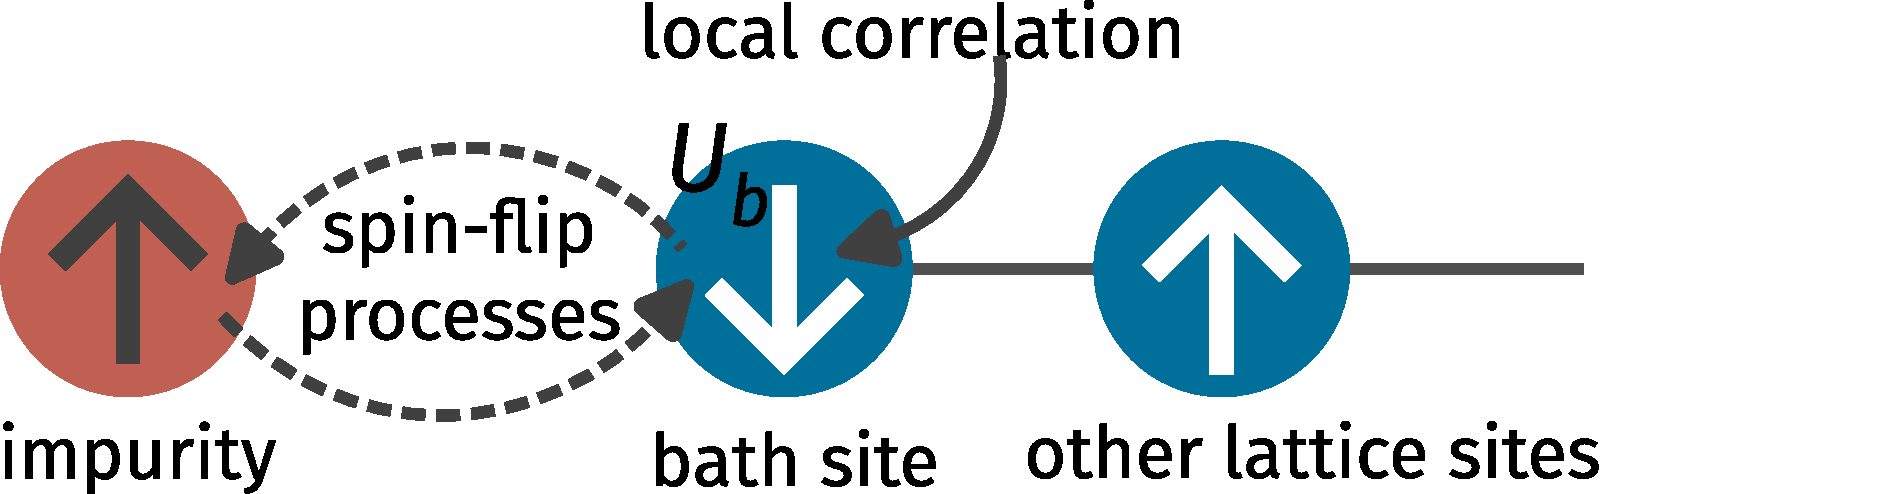
\includegraphics[width=\textwidth]{zeromode_bare.pdf}\\
\end{minipage}
}
\only<2>{
URG equations show that an \alert{attractive} \(U_b\) competes with \(J\):
\[\Delta J \sim J^2 + 4U_b J \implies \text{\alert{phase transition} at }J = -4U_b\]
This happens because the zeroth site is \alert{frustrated}.

\vspace*{\fill}

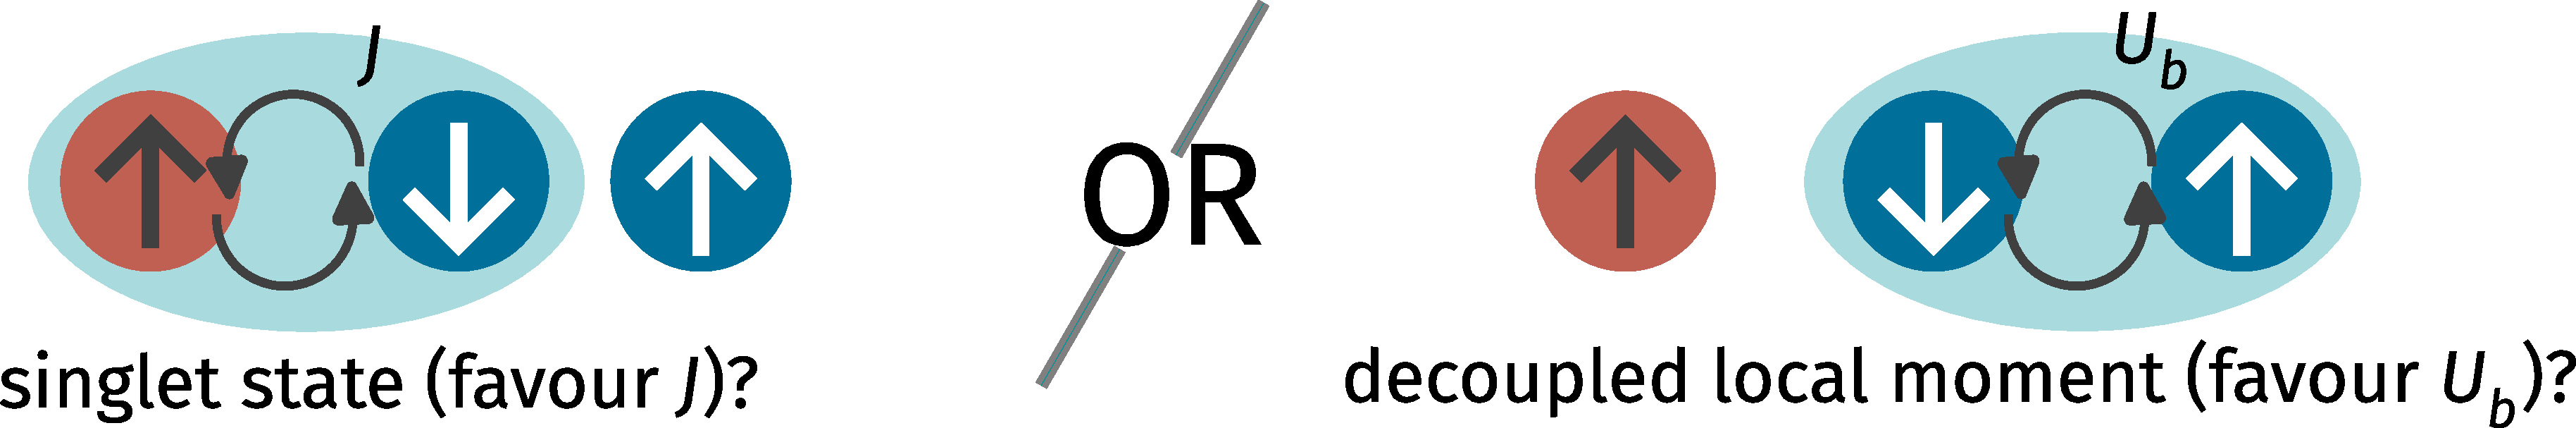
\includegraphics[width=\textwidth]{frustration.pdf}\\
}
\end{frame}

\begin{frame}{Nature of the transition}
\only<1>{
\begin{minipage}{0.4\textwidth}
Correlation functions show \\\alert{discontinuity} across transition.\\[10pt]
Impurity correlations vanish, bath correlations become non-zero.\\[10pt]
\end{minipage}
\hspace*{\fill}
\begin{minipage}{0.5\textwidth}
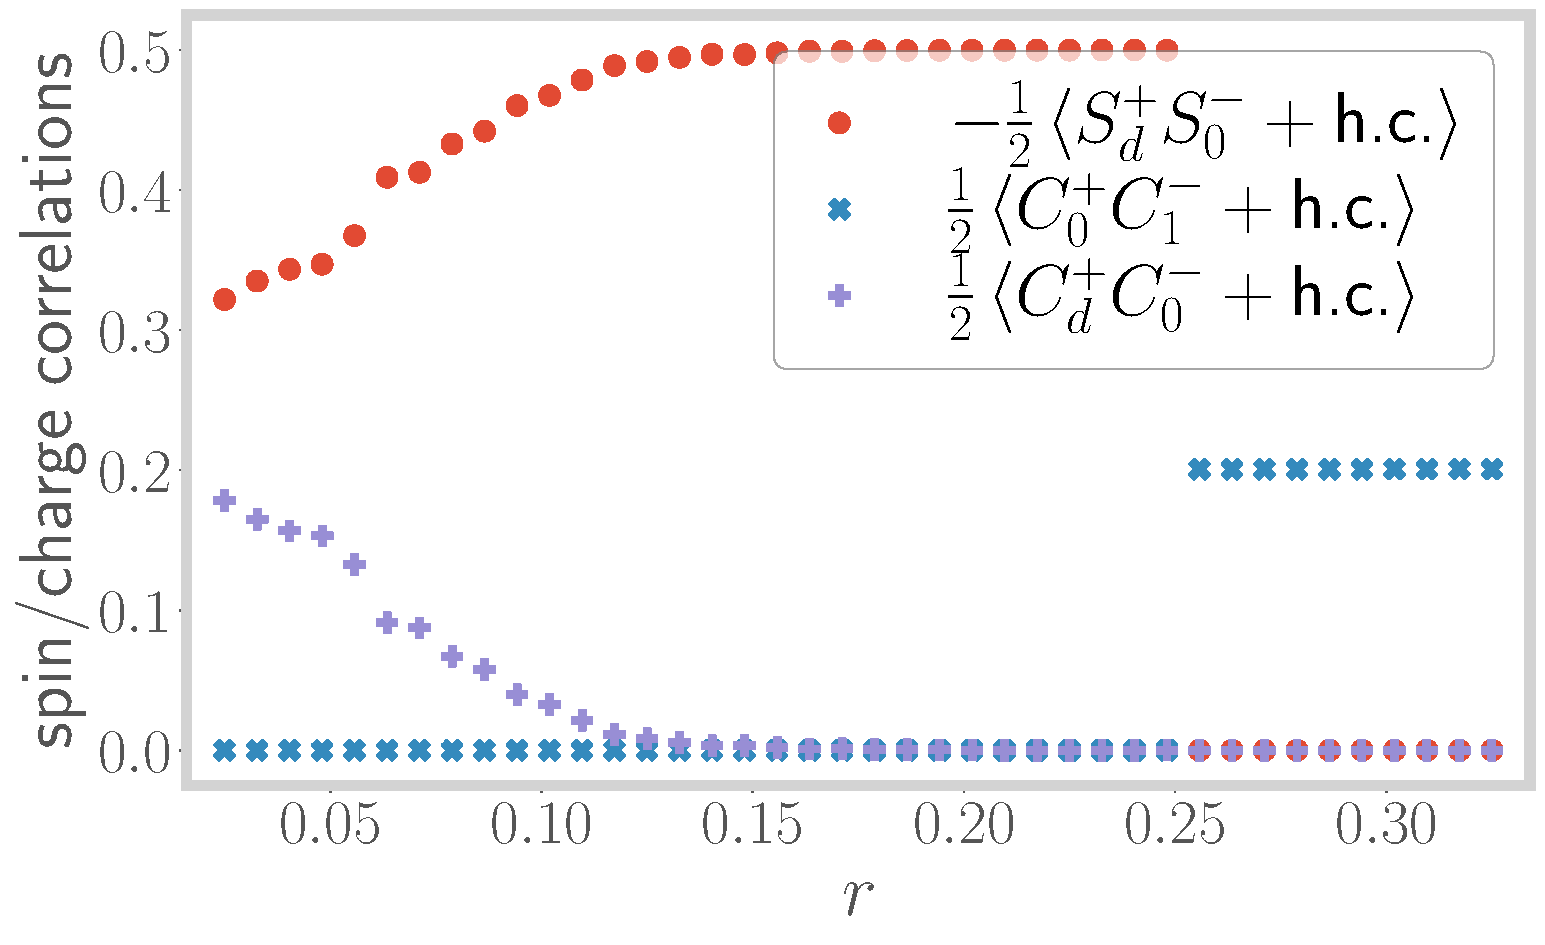
\includegraphics[width=\textwidth]{spin-charge-corr-full.pdf}
\end{minipage}

\vspace*{\fill}
Shows that \alert{pairing correlations} in the bath are responsible for the transition.
}
\only<2>{
\begin{minipage}{0.5\textwidth}
Manifests as a \alert{level crossing} in the zero bandwidth problem.\\[10pt]
The state precisely at the transition is special:
\begin{itemize}
	\item non-Fermi liquid excitations
	\item \alert{fractional} impurity magnetisation and occupancy
\end{itemize}
\end{minipage}
\hspace*{\fill}
\begin{minipage}{0.4\textwidth}
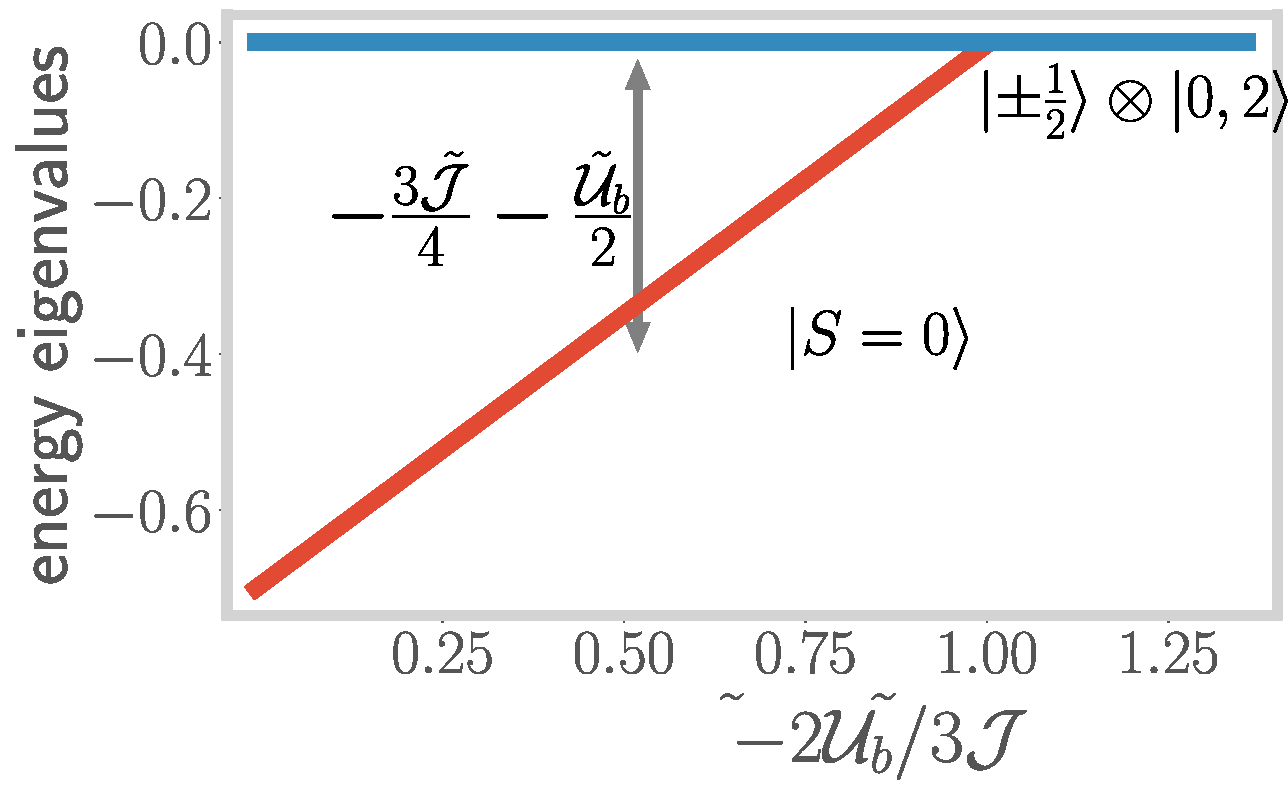
\includegraphics[width=\textwidth]{twosite_spectrum.pdf}
\end{minipage}
}
\end{frame}

\section{Concluding remarks and takeaways}
\subsection{~}
\begin{frame}{Concluding remarks}
We have answered the questions posed at the beginning:\\
\vspace*{\fill}

\begin{itemize}[<+->]
	\item obtained the effective theory for the Kondo cloud,\\[10pt]
	\item learnt multiple ways of hampering the Kondo effect, and\\[10pt]
	\item studied the various phases arising from this.
\end{itemize}
\vspace*{\fill}

\hspace*{\fill}
\only<1->{
\centering
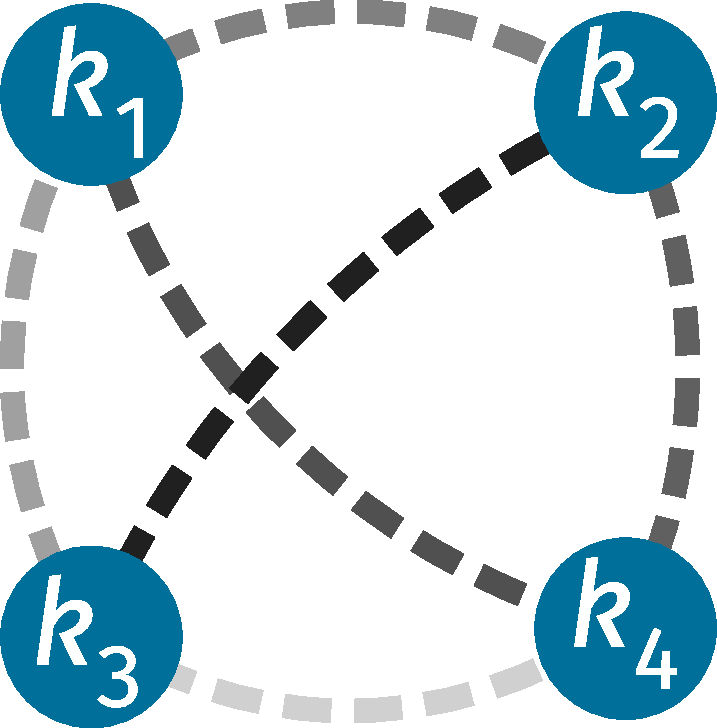
\includegraphics[width=0.2\textwidth]{takeaway2.pdf}
}
\hspace*{\fill}
\only<2->{
\centering
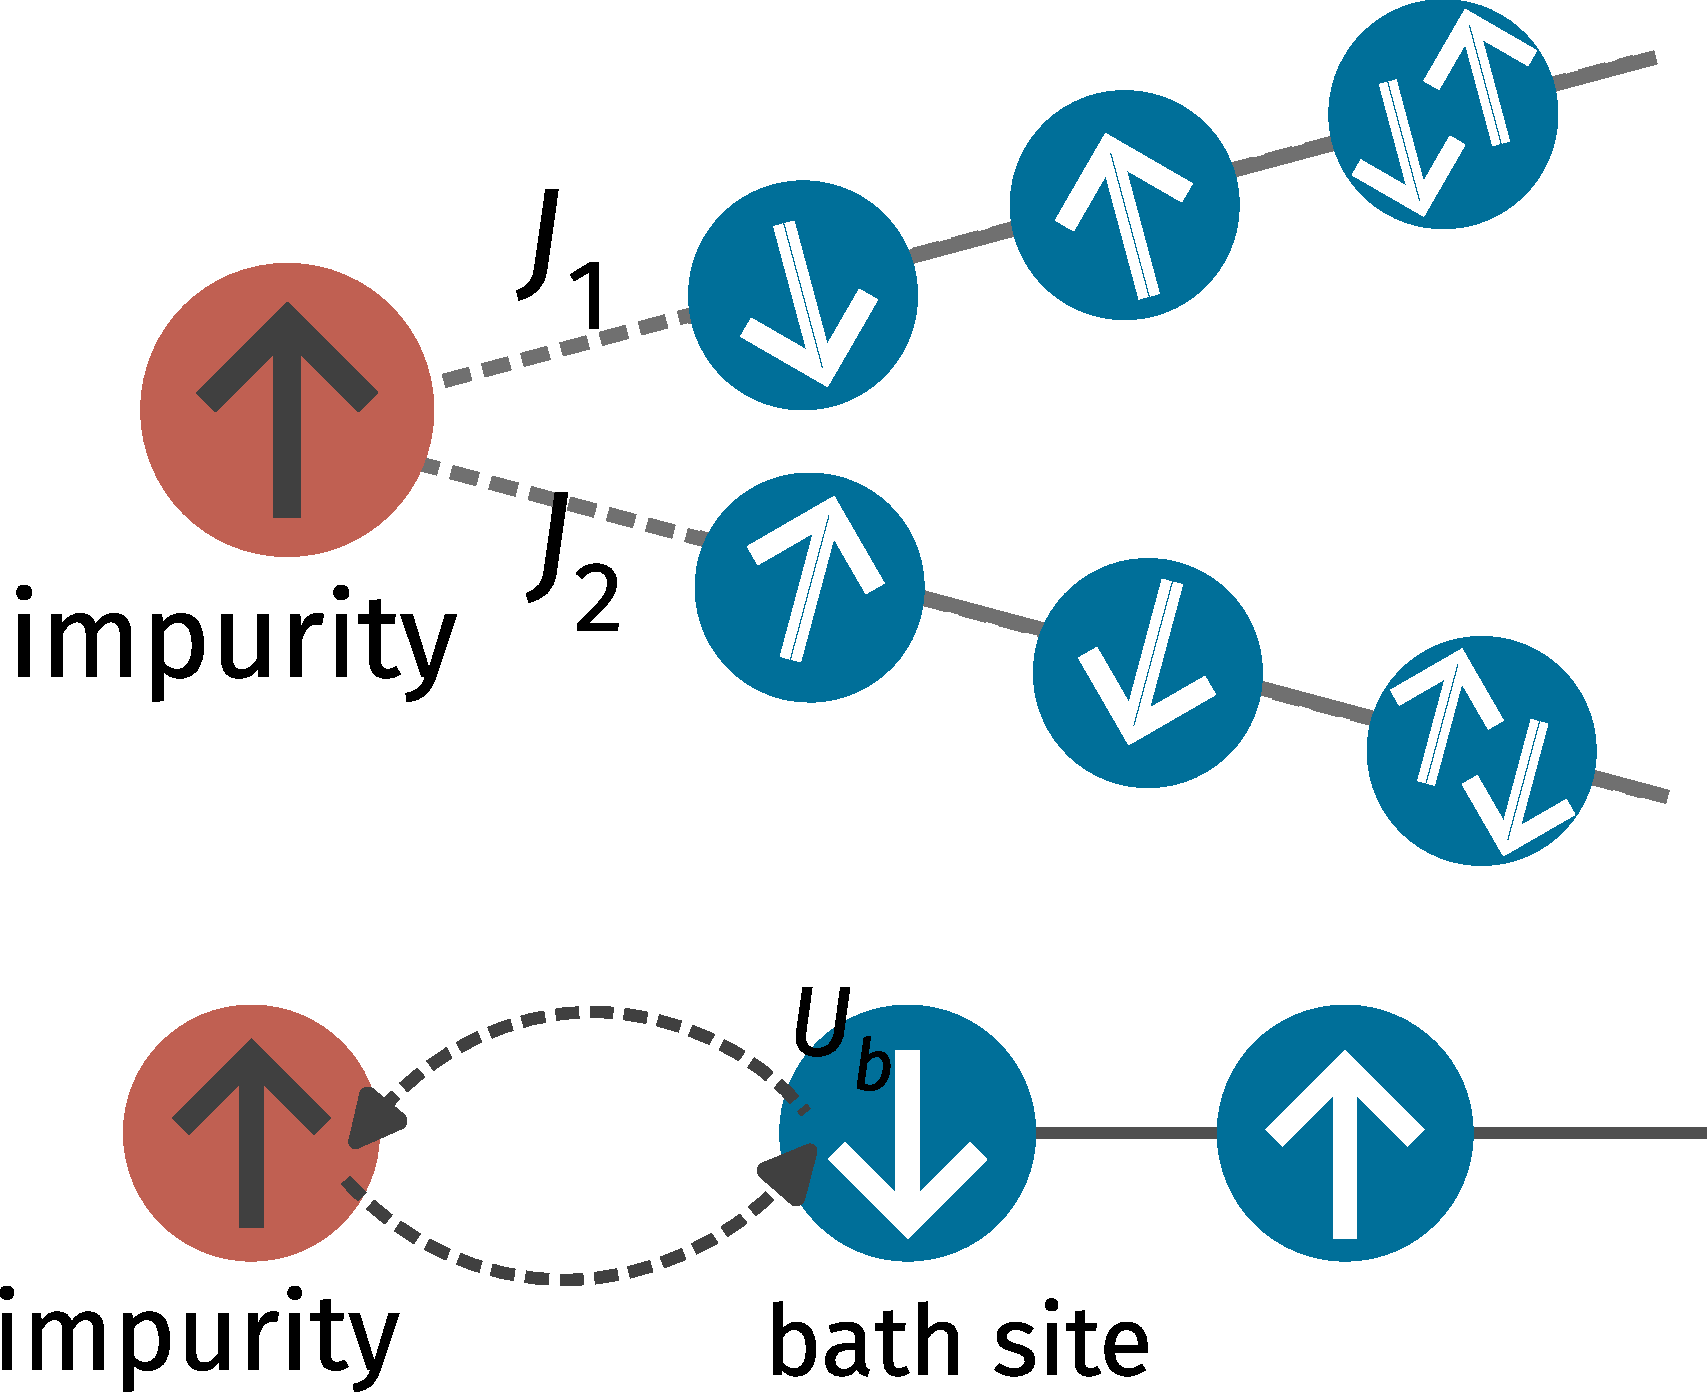
\includegraphics[width=0.3\textwidth]{takeaway1.pdf}
}
\hspace*{\fill}
\only<3>{
\centering
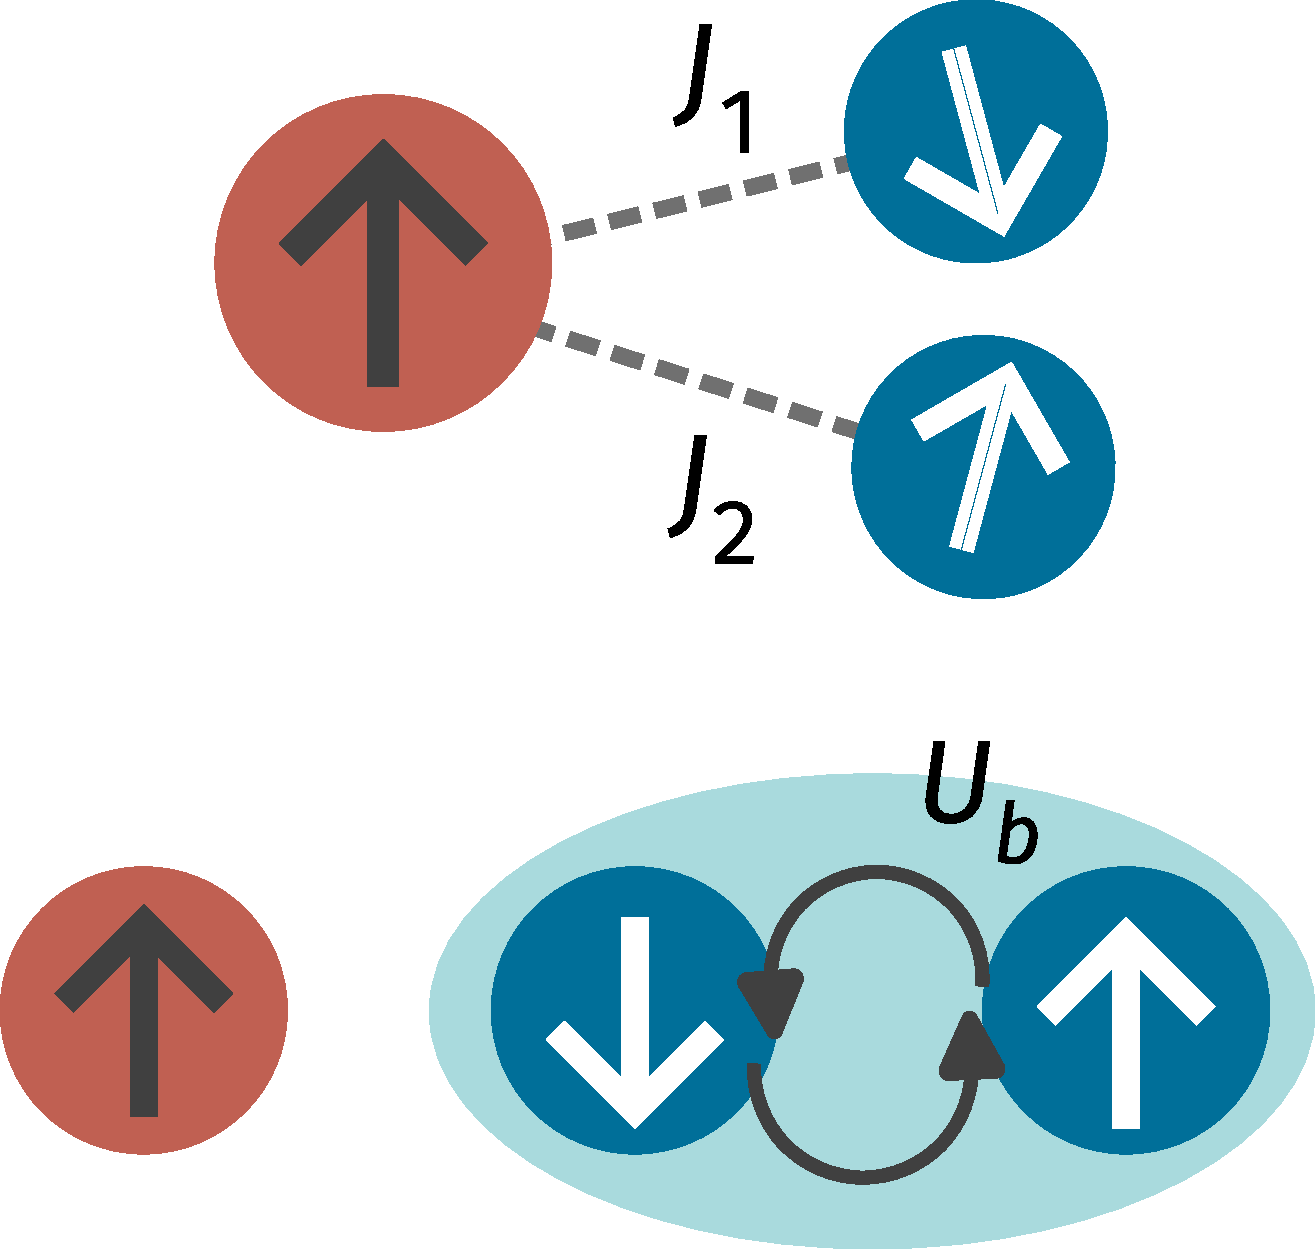
\includegraphics[width=0.25\textwidth]{takeaway3.pdf}
}
\hspace*{\fill}
\end{frame}
\begin{frame}{Takeaways}
	\begin{itemize}[<+->]
	\item Our analyses often link entanglement measures with correlations, providing bridges between the worlds of condensed matter and quantum information.\\[10pt]
	\only<1>{
	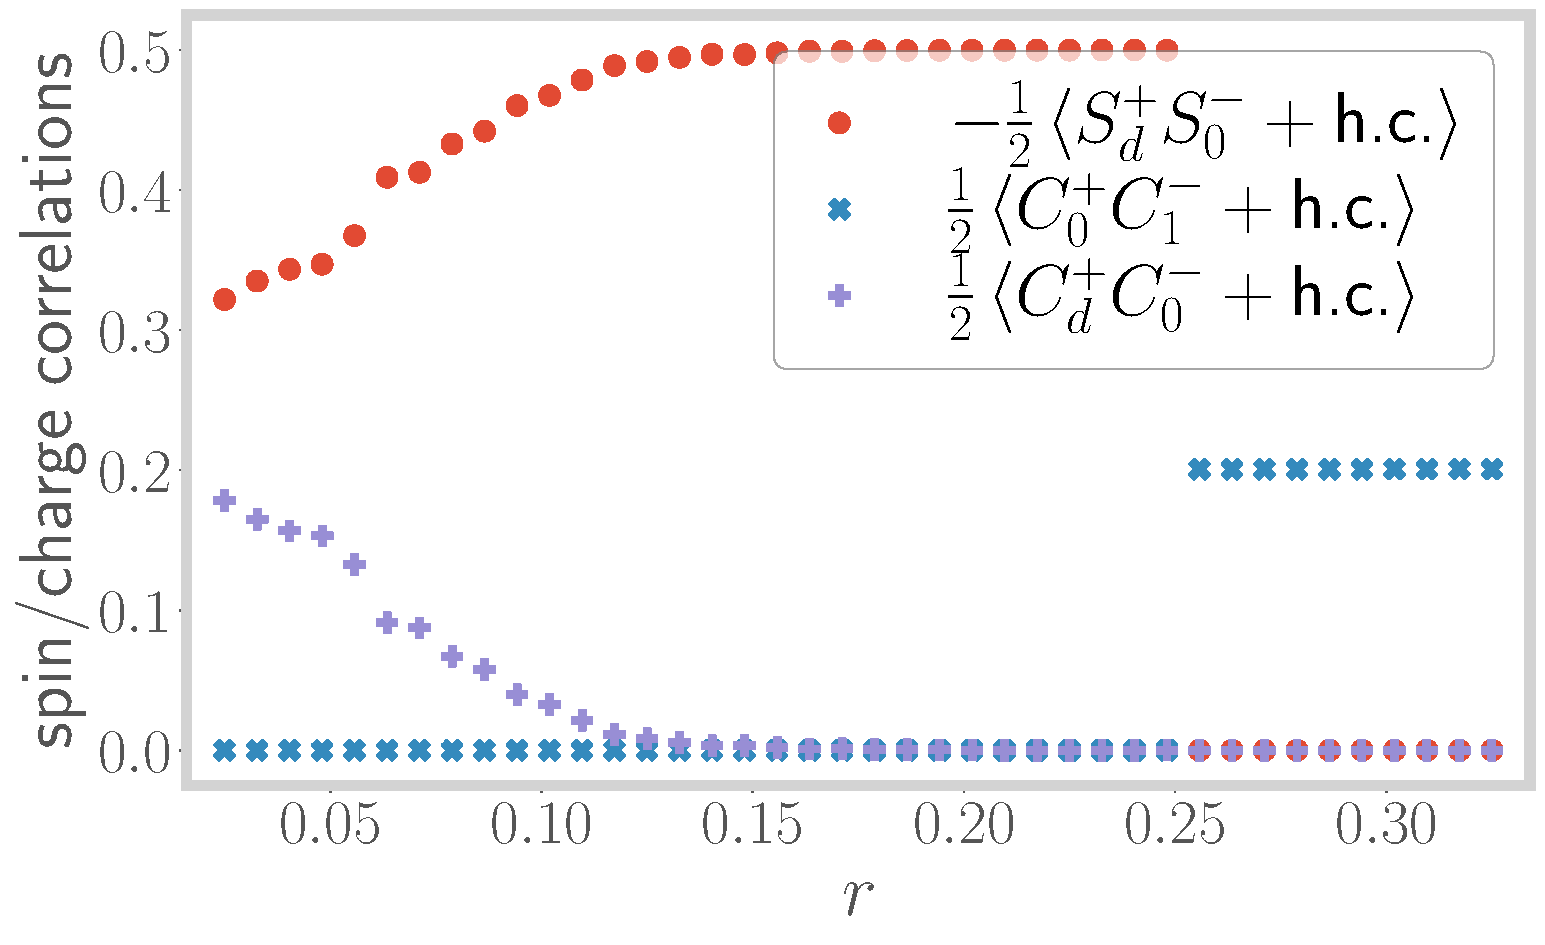
\includegraphics[width=0.45\textwidth]{spin-charge-corr-full.pdf}
	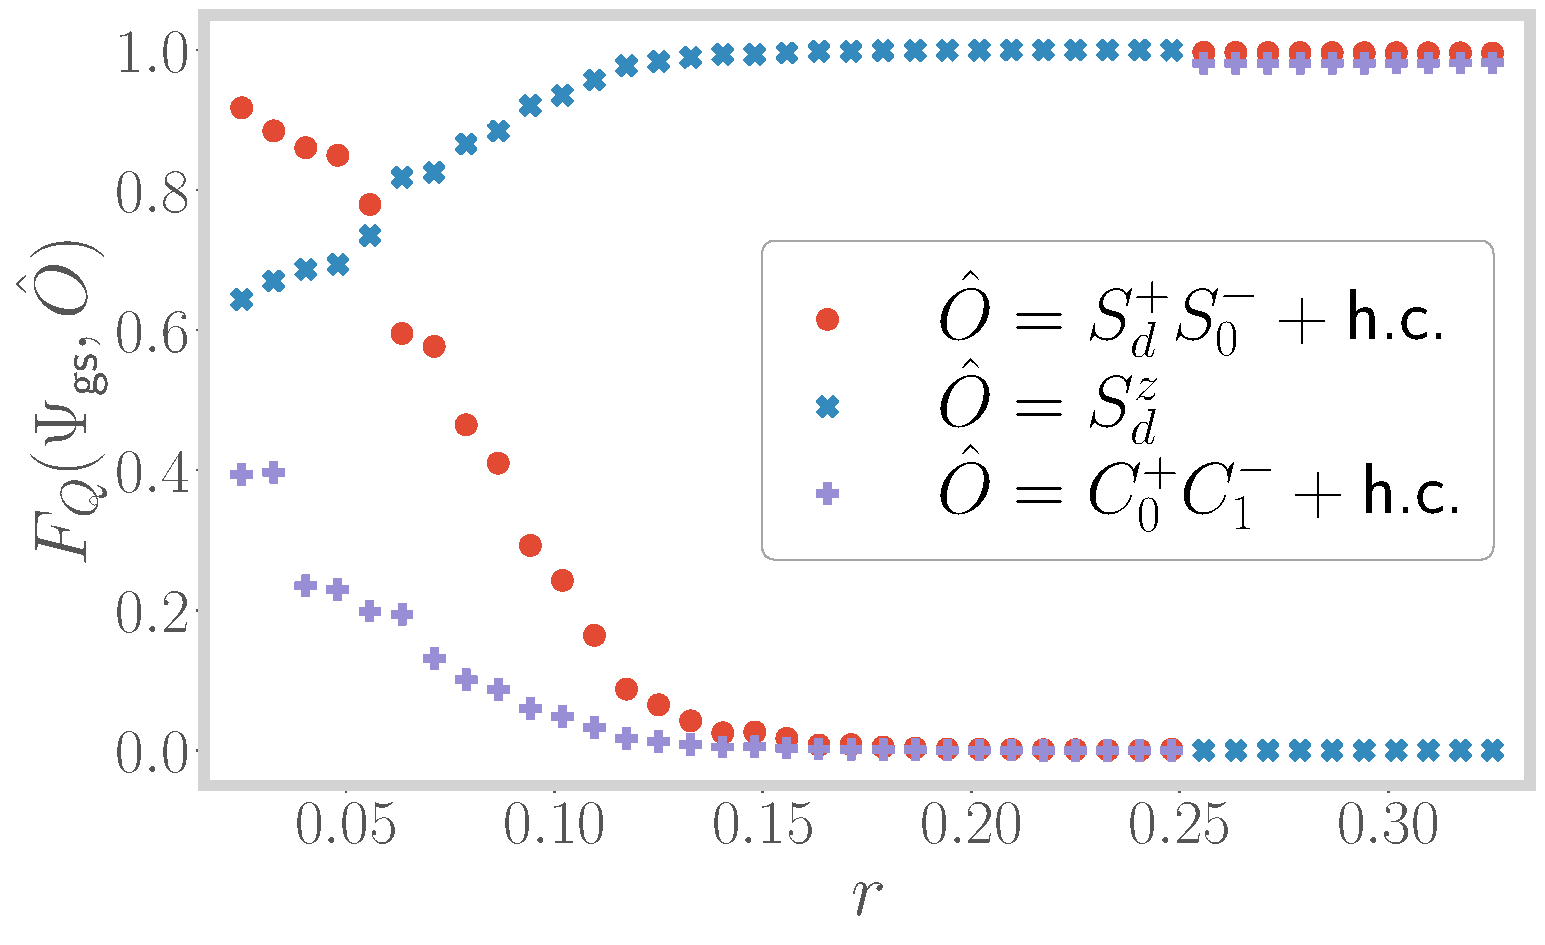
\includegraphics[width=0.45\textwidth]{QFI.pdf}
	}
	\item Models of Kondo breakdown can be used to study the effects of measurement on a system coupled to a bath.\\[10pt]
	\only<2>{
	\centering
	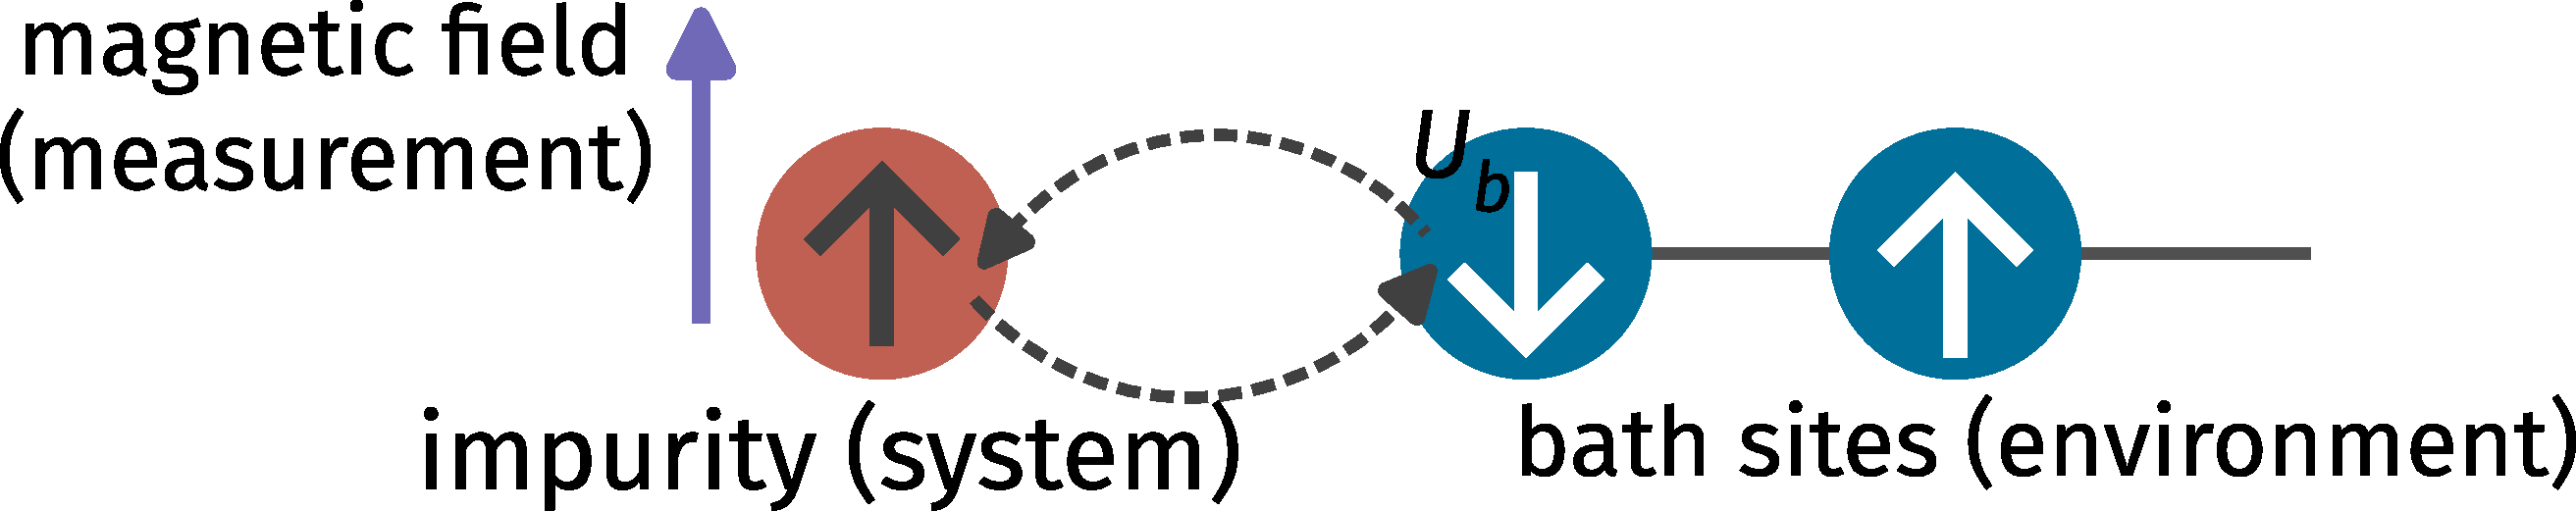
\includegraphics[width=0.65\textwidth]{measurement.pdf}
	}
	\item The Kondo model with attractive \(U_b\) term has applications in studying the physics of Mott transitions.
\end{itemize}
\end{frame}

\section{That's all!}
\subsection{Thanks to everyone.}
\end{document}
